%% Dissertação de Mestrado — UFPE / CIn
%% Programa de Pós-Graduação em Ciência da Computação
%% Padrão baseado no modelo oficial (versão 07.10.2020 v1.3)

\documentclass[12pt, a4paper, oneside]{report}

%% Pacotes básicos
\usepackage[utf8]{inputenc}
\usepackage[T1]{fontenc}
\usepackage[brazil]{babel}
\usepackage{lmodern}
\usepackage[expansion=false]{microtype} % expansion disabled to cut Overleaf free-tier compile time
\usepackage{geometry}
\usepackage{setspace}
\usepackage{indentfirst}
\usepackage{graphicx}
\usepackage{float}
\graphicspath{{figuras/}}
\usepackage{booktabs}
\usepackage{tabularx}
\usepackage{amsmath}
\usepackage{amssymb}
\usepackage{listings}
\usepackage{xcolor}
\lstdefinestyle{pycode}{
  basicstyle=\ttfamily\scriptsize,
  keywordstyle=\color{blue!60!black}\bfseries,
  commentstyle=\color{gray},
  stringstyle=\color{orange!70!black},
  numbers=left,
  numberstyle=\tiny\color{gray},
  numbersep=6pt,
  frame=single,
  breaklines=true,
  showstringspaces=false,
  language=Python,
  tabsize=2,
  captionpos=b
}
\usepackage{tikz}
\usetikzlibrary{positioning,arrows.meta,fit,backgrounds}
\usepackage{hyperref}
\usepackage[alf]{abntex2/abntex2cite}
\providecommand{\abntnextkey}{}
\usepackage{fancyhdr}
\usepackage{emptypage}
\usepackage{epigraph}
\setlength{\epigraphwidth}{0.62\textwidth}
\renewcommand{\epigraphflush}{flushright}
\renewcommand{\epigraphrule}{0pt}

%% Margens ABNT
\geometry{
  top=3cm, bottom=2cm,
  left=3cm, right=2cm
}

%% Espaçamento 1.5
\onehalfspacing

%% Numeração de página no topo direito
\pagestyle{fancy}
\fancyhf{}
\fancyhead[R]{\thepage}
\renewcommand{\headrulewidth}{0pt}

%% Formatação de capítulos: negrito, caixa alta
\usepackage{titlesec}
\titleformat{\chapter}[block]
  {\normalfont\bfseries\large}
  {\thechapter}
  {1em}
  {\MakeUppercase}

\titleformat{\section}[block]
  {\normalfont\normalsize}
  {\thesection}
  {1em}
  {\MakeUppercase}

\titleformat{\subsection}[block]
  {\normalfont\normalsize\bfseries}
  {\thesubsection}
  {1em}
  {}

%% Profundidade do sumário
\setcounter{tocdepth}{2}

%% Hiperlinks discretos
\hypersetup{
  colorlinks=true,
  linkcolor=black,
  citecolor=black,
  urlcolor=black
}

%% ──────────────────────────────────────────────────────────────────────────────
\begin{document}

%% Elementos pré-textuais
\pagenumbering{roman}
\pagestyle{empty}

\begin{titlepage}
\centering

\vspace*{1cm}


\includegraphics[width=2.2cm]{figuras/ufpe_logo.png}\\[0.5cm]

{\normalsize UNIVERSIDADE FEDERAL DE PERNAMBUCO}\\
{\normalsize CENTRO DE INFORMÁTICA}\\
{\normalsize PROGRAMA DE PÓS-GRADUAÇÃO EM CIÊNCIA DA COMPUTAÇÃO}

\vspace{3cm}

{\normalsize Eduardo Wanderley}

\vspace{3cm}

{\normalsize
Um Framework de Orquestração de Experimentos para\\
Repetibilidade de Navegação Autônoma com\\
Robôs Móveis em ROS~2
}

\vfill

{\normalsize Recife}\\
{\normalsize 2026}

\end{titlepage}

\begin{titlepage}
\centering

{\normalsize Eduardo Wanderley}

\vspace{3cm}

{\normalsize
Um Framework de Orquestração de Experimentos para\\
Repetibilidade de Navegação Autônoma com\\
Robôs Móveis em ROS~2
}

\vspace{3cm}

\hfill
\begin{minipage}{0.5\textwidth}
\small
Trabalho apresentado ao Programa de Pós-Graduação em Ciência da Computação do Centro de Informática da Universidade Federal de Pernambuco como requisito parcial para obtenção do grau de Mestre em Ciência da Computação.

\vspace{0.5cm}
\textbf{Área de Concentração}: Sistemas de Computação e Robótica

\vspace{0.5cm}
\textbf{Orientador}: Prof. Breno Miranda
\end{minipage}

\vfill

{\normalsize Recife}\\
{\normalsize 2026}

\end{titlepage}


\cleardoublepage
\centerline{\textbf{FICHA CATALOGRÁFICA}}
\vspace{2cm}
\noindent [A ser preenchida pela Biblioteca Central — após aprovação]

\cleardoublepage
\centerline{\textbf{FOLHA DE APROVAÇÃO}}
\vspace{2cm}
\noindent [A ser inserida pela Secretaria do Programa de Pós-Graduação]

\cleardoublepage
\vspace*{\fill}
\begin{flushright}
\textit{À minha família,\\
por tornarem cada desafio possível.}
\end{flushright}


\cleardoublepage
\chapter*{AGRADECIMENTOS}
\addcontentsline{toc}{chapter}{AGRADECIMENTOS}

[A ser preenchido pelo autor.]


\cleardoublepage
\vspace*{\fill}
\begin{flushright}
\begin{minipage}{0.6\textwidth}
\small\itshape
``A repetibilidade não é uma limitação da ciência;\\
é a sua condição de existência.''

\vspace{0.3cm}
--- Karl Popper, \textit{A Lógica da Pesquisa Científica}, 1934
\end{minipage}
\end{flushright}


\cleardoublepage
\chapter*{ABSTRACT}
\addcontentsline{toc}{chapter}{ABSTRACT}

Reproducibility is a cornerstone of experimental science, yet mobile robotics research
has long struggled to establish it in practice. Setting up a navigation experiment,
recording sensor data across multiple runs, and comparing the resulting trajectories
quantitatively demands a level of infrastructure that most robotics labs build informally,
once per project, with no reuse in mind. This dissertation presents a framework that
makes those steps explicit, automated, and transferable.

The proposed system — called \textit{Fleet UI} — orchestrates autonomous navigation
experiments with one or more mobile robots running ROS~2 Jazzy and the Nav2 navigation
stack. A role-based architecture separates units into \textit{MUUT} (Mobile Unit Under
Test), which executes and records routes, and \textit{FUUT} (Fixed Unit Under Test),
which observes from a fixed position. This separation allows the same physical testbed
to serve fundamentally different experimental designs without changing the software layer.

The record--replay protocol forms the experimental nucleus: a baseline route is defined
by navigating a set of waypoints; the orchestrator stores the visited poses; subsequent
replay runs reproduce those poses using Nav2's \texttt{FollowWaypoints} action.
Sensor bags in MCAP format capture LiDAR, wheel odometry, IMU, and SLAM-estimated pose
at each run. Offline analysis computes pairwise Root Mean Square Error (RMSE) between
trajectories resampled on a normalized time grid, producing trajectory overlays and
repeatability metrics.

Quantitative validation, carried out in Gazebo Harmonic simulation with a single
TurtleBot4 Standard unit, used a clean baseline and ten independent replay executions.
Each replay was started from the same initial state by fully relaunching the simulator,
the Nav2 stack, and the data collection nodes, ensuring that recorded odometry started
at practically the same point in every run. The campaign achieved a mean RMSE of
3.35\,cm between each replay and the reference run, with a maximum of 4.76\,cm, over
trajectories with a mean length of 0.826\,m. The mean final endpoint error was
1.64\,cm (maximum 3.26\,cm), and the mean duration was 17.51\,s with a standard
deviation of 0.36\,s. These results are comfortably below Nav2's default 25\,cm goal
tolerance; the architecture supports multiple units, but empirical evaluation of
simultaneous multi-robot fleet scenarios was not conducted in this dissertation. A web
interface built on React and FastAPI allows researchers to define experiments, monitor
sensor state, and visualise trajectories on the SLAM map without direct exposure to the
ROS~2 command line.

\vspace{0.5cm}
\noindent\textbf{Keywords}: autonomous navigation; path repeatability; mobile robot fleet;
ROS~2; Nav2; SLAM; sensor data collection; experimental framework.


\cleardoublepage
\chapter*{RESUMO}
\addcontentsline{toc}{chapter}{RESUMO}

A reprodutibilidade é um pilar do método científico, mas a pesquisa em robótica móvel
raramente a alcança de forma sistemática. Configurar um experimento de navegação,
registrar dados sensoriais ao longo de múltiplas execuções e comparar as trajetórias
resultantes com rigor quantitativo exige uma infraestrutura que a maioria dos laboratórios
constrói de forma improvisada, específica para cada projeto, sem possibilidade de reuso.
Esta dissertação apresenta um framework que torna essas etapas explícitas, automatizadas
e transferíveis.

O sistema proposto --- denominado \textit{Fleet UI} --- orquestra experimentos de navegação
autônoma com um ou mais robôs móveis operando sob ROS~2 Jazzy e a pilha de navegação Nav2.
Uma arquitetura baseada em papéis separa as unidades em \textit{MUUT} (Mobile Unit Under
Test), responsável pela execução e gravação das rotas, e \textit{FUUT} (Fixed Unit Under
Test), que observa o cenário de uma posição fixa. Essa separação permite que o mesmo
testbed físico sirva a diferentes desenhos experimentais sem modificação da camada de software.

O protocolo de gravação--reprodução constitui o núcleo experimental: uma rota é definida
por navegação sequencial de waypoints; o orquestrador armazena as poses atingidas; as
execuções subsequentes de replay reproduzem essas poses via a ação \texttt{FollowWaypoints}
do Nav2. Bags de sensores no formato MCAP capturam LiDAR, odometria de roda, IMU e
pose estimada pelo SLAM em cada execução. A análise \textit{offline} calcula o
\textit{Root Mean Square Error} (RMSE) entre trajetórias reamostradas em tempo
normalizado, gerando sobreposições visuais e métricas de repetibilidade.

A validação quantitativa, realizada em simulação Gazebo Harmonic com uma única
unidade TurtleBot4 Standard, utilizou uma baseline limpa e dez execuções independentes
de replay. Cada replay foi iniciado a partir do mesmo estado por relançamento completo
da simulação, da pilha Nav2 e dos nós de coleta, garantindo que a odometria registrada
começasse praticamente no mesmo ponto em todas as execuções. A campanha obteve RMSE
médio de 3,35\,cm entre cada replay e a execução de referência, com máximo de
4,76\,cm, em trajetórias com comprimento médio de 0,826\,m. O erro final médio foi de
1,64\,cm (máximo de 3,26\,cm), e a duração média foi de 17,51\,s com desvio-padrão de
0,36\,s. Esses resultados ficam confortavelmente abaixo da tolerância padrão do Nav2 de
25\,cm; a arquitetura suporta múltiplas unidades, mas a avaliação empírica de cenários
com frota simultânea não foi conduzida nesta dissertação. Uma interface web em React e
FastAPI permite que pesquisadores definam experimentos, monitorem o estado dos sensores
e visualizem trajetórias sobre o mapa SLAM sem exposição direta à linha de comando do
ROS~2.

\vspace{0.5cm}
\noindent\textbf{Palavras-chave}: navegação autônoma; repetibilidade de trajetórias;
frota de robôs móveis; ROS~2; Nav2; SLAM; coleta de dados sensoriais; framework experimental.


\cleardoublepage
\listoffigures
\addcontentsline{toc}{chapter}{LISTA DE FIGURAS}

\cleardoublepage
\listoftables
\addcontentsline{toc}{chapter}{LISTA DE TABELAS}

\cleardoublepage
\tableofcontents

%% Elementos textuais
\cleardoublepage
\pagenumbering{arabic}
\pagestyle{fancy}

\chapter{Introdução}
\label{chap:introducao}

\epigraph{\itshape ``A ciência avança um funeral de cada vez --- não porque os cientistas
mudam de ideia, mas porque as práticas experimentais que permitiam verificar isso
finalmente chegam ao alcance de todos.''}{\normalfont --- adaptado de Max Planck}

\section{Contexto e Motivação}
\label{sec:motivacao}

A robótica autônoma atravessa um momento singular em sua história. A convergência de
plataformas de software maduras --- especialmente o ROS~2 \cite{macenski2022ros2}
--- com hardware acessível e simuladores de alta fidelidade tornou possível, pela
primeira vez, que grupos de pesquisa sem grandes laboratórios físicos conduzam
experimentos de navegação com rigor comparável ao de instituições bem equipadas.
O que antes exigia uma sala climatizada, técnicos especializados e robôs industriais
de alto custo hoje pode ser realizado com um TurtleBot4, um computador convencional
e software inteiramente open-source.

Esse nivelamento de acesso, porém, não veio acompanhado de um nivelamento
metodológico equivalente. Enquanto os componentes técnicos se tornaram mais acessíveis,
os procedimentos que tornam um experimento reprodutível permaneceram informais,
específicos por equipe, raramente documentados e quase nunca transferíveis. A questão
não é mais \textit{se} um pesquisador consegue fazer um robô navegar --- é se consegue
fazer isso de uma forma que outro pesquisador possa verificar.

A comunidade de robótica reconhece essa lacuna metodológica há mais de uma
década \cite{bonsignorio2015}. Esta dissertação distingue, desde este parágrafo
em diante, dois conceitos que a literatura de ciência experimental frequentemente
trata como sinônimos, mas que não o são \cite{acm2020badging}. \textbf{Repetibilidade} é a capacidade do
mesmo sistema, no mesmo ambiente, sob as mesmas condições, de produzir
resultados equivalentes em execuções sucessivas. \textbf{Reprodutibilidade}, em
sentido mais forte, é a capacidade de um investigador independente, em outro
ambiente, obter resultados equivalentes a partir do mesmo artefato de pesquisa
--- código, dados e protocolo publicados \cite{amigoni2010}. Repetibilidade é
condição necessária, mas não suficiente, para reprodutibilidade: um sistema
pode ser perfeitamente repetível em um único laboratório e, ainda assim, nunca
ter sido reproduzido por ninguém fora dele.

Na prática, em robótica móvel, garantir repetibilidade significa assegurar que
o robô: (i) parta da mesma pose inicial em todas as execuções; (ii) percorra o
mesmo trajeto usando a mesma estratégia de navegação; (iii) tenha os dados de
todos os sensores coletados de forma síncrona e com a mesma configuração; e
(iv) tenha as trajetórias resultantes comparadas por um método que não
introduza vieses de análise. Cada um desses requisitos, isoladamente, é
simples. Satisfazê-los simultaneamente, de forma automática e reutilizável, é
onde a literatura apresenta uma lacuna persistente --- e é precisamente
repetibilidade, nesse sentido preciso, o que esta dissertação avalia
empiricamente (Capítulos~\ref{chap:avaliacao} e~\ref{chap:resultados}). O
framework proposto busca \emph{favorecer} reprodutibilidade --- por meio de
código aberto, protocolo documentado e artefatos de saída estruturados
(Seção~\ref{sec:rel_reprodutibilidade}) --- mas essa dissertação não conduziu
nem observou replicação independente por outro pesquisador ou laboratório;
a Seção~\ref{sec:repro_vs_repet} retoma essa distinção à luz dos resultados
obtidos.

Essa lacuna tem custos concretos. Quando um artigo reporta que ``o robô navegou com
erro médio de 8\,cm'', sem especificar se essa é a média de 3 ou 30 execuções, se o
desvio padrão foi medido, ou se a comparação com trabalhos anteriores usa a mesma
métrica, a contribuição científica se torna não verificável. A acumulação de
resultados não reprodutíveis na literatura não é apenas um problema acadêmico
--- é um obstáculo para a transferência de tecnologia para aplicações industriais
que dependem de garantias comportamentais precisas.

\section{O Problema Central: Crise de Orquestração Experimental}
\label{sec:problema}

Esta dissertação identifica e nomeia um problema específico que perpassa a robótica
experimental contemporânea: a \textbf{crise de orquestração experimental}. Trata-se
da dificuldade estrutural em coordenar, de forma automática e repetível, as múltiplas
camadas de um experimento de navegação autônoma --- inicialização do ambiente de
simulação, ativação da pilha de navegação com tempo de espera correto, definição e
execução de rotas, coleta síncrona de múltiplos sensores com políticas de QoS adequadas,
e análise quantitativa comparável entre execuções.

Cada uma dessas camadas possui sua própria curva de aprendizado. O modelo de lifecycle
do ROS~2 \cite{macenski2022ros2} exige que os nós de navegação sejam ativados na
sequência correta antes que qualquer comando seja enviado. As políticas de QoS de
tópicos como \texttt{/\allowbreak scan} (BEST\_EFFORT), \texttt{/\allowbreak pose} (RELIABLE) e
\texttt{/\allowbreak amcl\_\allowbreak pose} (TRANSIENT\_LOCAL) determinam se os dados serão efetivamente
gravados nos bags ou silenciosamente descartados. O protocolo de ações do Nav2
\cite{macenski2020marathon} opera de forma assíncrona, e uma chamada prematura ao
servidor de ações resulta em timeout sem mensagem de erro clara. O SLAM Toolbox
\cite{macenski2021slam} precisa de scans suficientes antes de publicar uma estimativa
confiável de mapa, e o intervalo correto varia com o ambiente.

Nenhum desses problemas é intratável. Todos são resolvidos por equipes experientes,
individualmente, a cada novo experimento. O problema é que essa solução acontece
de forma invisível, em scripts não publicados, em notebooks Jupyter apagados ao fim
do projeto, em conversas de corredor que nunca entram na seção de metodologia do artigo.
O conhecimento que torna um experimento bem-feito permanece tácito e não transferível.

\section{O Papel da Robótica de Frota nos Experimentos Modernos}
\label{sec:frota}

A tendência recente em robótica de serviço e logística autônoma é operar não um
robô isolado, mas frotas de agentes coordenados \cite{macenski2022ros2}. Em um
testbed experimental, isso cria possibilidades metodológicas que um único robô
não oferece: enquanto uma Unidade Móvel sob Teste (MUUT) percorre sua rota, uma
Unidade Fixa sob Teste (FUUT) pode observar a mesma cena de um ângulo externo,
coletando dados independentes que funcionam como fonte de verdade alternativa.

Essa dualidade de perspectivas --- endógena (o que o robô vê de si mesmo) e exógena
(o que um observador fixo vê do robô) --- enriquece substancialmente a análise de
repetibilidade. Pequenas variações de trajetória que seriam invisíveis à odometria
interna do MUUT podem ser capturadas pelos scans do FUUT como variações na posição
relativa do robô ao passar em frente ao sensor.

O framework proposto nesta dissertação formaliza esse design experimental com uma
arquitetura de papéis explícita, garantindo que as regras de cada tipo de unidade
sejam verificadas em software --- não apenas documentadas no protocolo.

\section{Escopo e Restrições}
\label{sec:escopo}

Esta dissertação foca na navegação 2D de robôs diferenciais em ambientes fechados,
usando o TurtleBot4 Standard com RPLIDAR S2 como plataforma de referência. Todos
os experimentos de validação foram conduzidos em simulação Gazebo Harmonic, o que
garante condições perfeitamente controladas mas abstrai os fenômenos físicos de
superfícies reais, slip de roda e variação de calibração de sensores ao longo do
tempo.

As métricas adotadas --- RMSE, erro de endpoint e consistência temporal --- são
métricas espaciotemporais clássicas para avaliação de navegação \cite{amigoni2010},
mas não capturam aspectos como consumo energético, desgaste mecânico ou robustez
a falhas de comunicação. Essas dimensões constituem extensões naturais do trabalho,
identificadas na seção de trabalhos futuros.

\section{Objetivos}
\label{sec:objetivos}

O objetivo geral desta dissertação é projetar e implementar um framework
open-source de orquestração de experimentos de repetibilidade de navegação
autônoma para frotas de robôs móveis em ROS~2, e avaliar empiricamente sua
capacidade de produzir execuções repetíveis --- avaliação que, como detalhado
no Capítulo~\ref{chap:avaliacao}, foi conduzida com uma única unidade móvel; a
extensão dessa avaliação para operação simultânea de múltiplos robôs é tratada
como trabalho futuro (Seção~\ref{sec:futuros}).

Os objetivos específicos são:

\begin{enumerate}
    \item Definir formalmente uma arquitetura de papéis experimentais (MUUT/FUUT/SU)
    que separe responsabilidades entre unidades móveis e fixas de forma explícita e
    verificável em software.

    \item Implementar serviços ROS~2 que abstraiam as ações Nav2 e a coleta síncrona
    de sensores em uma interface de alto nível, sem expor ao pesquisador os detalhes
    de QoS, lifecycle ou protocolo de ações.

    \item Desenvolver um protocolo de gravação--reprodução (record--replay) com
    garantias de consistência entre execuções, incluindo retorno automático ao ponto
    de partida e gravação de poses efetivamente atingidas.

    \item Construir uma interface web que permita configuração, execução e visualização
    de experimentos com waypoints clicáveis sobre o mapa SLAM ao vivo, sem necessidade
    de linha de comando.

    \item Validar o framework em dois cenários de simulação e reportar métricas de
    repetibilidade (RMSE inter-replay, RMSE vs. baseline, erro de endpoint e
    consistência temporal) como baseline empírico para trabalhos futuros.
\end{enumerate}


\section{Perguntas de Pesquisa e Hipóteses}
\label{sec:perguntas_pesquisa}

A partir dos objetivos específicos listados na Seção~\ref{sec:objetivos}, esta
dissertação formaliza quatro perguntas de pesquisa (PP), cada uma associada a
uma hipótese de trabalho (H) verificada empiricamente nos capítulos de
Avaliação e Resultados (Capítulos~\ref{chap:avaliacao} e~\ref{chap:resultados}).

\begin{description}
    \item[PP1 --- Automação de protocolo.] É possível automatizar integralmente
    o protocolo de gravação--reprodução de rotas em uma frota heterogênea de
    robôs ROS~2, sem intervenção manual entre fases, preservando a semântica
    de papéis experimentais (MUUT/FUUT/SU)?
    \textbf{H1}: um conjunto reduzido de serviços ROS~2 de alto nível
    (Seção~\ref{sec:orquestrador}), combinado a um script orquestrador de
    linha de comando, é suficiente para expressar qualquer protocolo de
    record--replay sem código adicional por experimento.

    \item[PP2 --- Repetibilidade mensurável.] Qual é o grau de repetibilidade
    espacial (RMSE) e temporal (CV$_t$) de execuções de replay sucessivas sobre
    a mesma rota, sob controlador e SLAM padrão do Nav2/SLAM Toolbox?
    \textbf{H2}: em condições de simulação controlada, o RMSE inter-replay é
    inferior a 30\,cm e o CV$_t$ é inferior a 10\%. Com $N=10$ replays na
    campanha final, esta dissertação caracteriza a variabilidade observada no
    cenário avaliado, sem generalizar esse comportamento para todas as rotas,
    ambientes ou configurações do Nav2 (Seção~\ref{sec:mppi}).

    \item[PP3 --- Persistência da repetibilidade fora do regime estritamente
    controlado.] A baixa variabilidade observada sob o protocolo controlado
    (mesma ação de navegação, pose inicial fixa, $N=10$ na campanha final) se
    mantém quando as condições de execução são menos controladas?
    \textbf{H3}: espera-se que execuções fora do protocolo formal --- sem
    controle explícito de ação de navegação, pose inicial e retorno ao ponto
    de partida entre réplicas --- apresentem RMSE e variabilidade de duração
    substancialmente maiores que a campanha controlada final. Esta dissertação não
    hipotetiza, a priori, uma causa única para essa diferença; a Seção
    ~\ref{sec:res_exp_complementares} discute evidência exploratória
    compatível com H3, mas insuficiente para atribuir causalidade específica,
    e a Seção~\ref{sec:ameacas} trata essa limitação como ameaça à validade
    de conclusão.

    \item[PP4 --- Custo de engenharia para o pesquisador.] O framework reduz
    o esforço de engenharia necessário para configurar e executar um
    experimento de repetibilidade, em comparação com a composição manual de
    chamadas Nav2/rosbag2 descrita informalmente na literatura correlata
    (Capítulo~\ref{chap:relacionados})?
    \textbf{H4}: a interface web e a camada de serviços ROS~2
    (Seção~\ref{sec:backend_web}) eliminam a necessidade de escrever código
    Python ou lançar comandos \texttt{ros2} manualmente para configurar,
    executar e analisar um experimento completo.
\end{description}

Este trabalho não formaliza PP2--PP4 como hipóteses estatísticas testadas por
inferência formal com poder amostral pré-calculado. Embora a campanha final
tenha $N=10$ replays, ela permanece restrita a uma única rota curta, uma única
plataforma simulada e uma única configuração de navegação, limitação reconhecida
explicitamente na Seção~\ref{sec:ameacas}. As hipóteses acima são tratadas,
portanto, como proposições descritivas a serem corroboradas ou refutadas pela
evidência empírica coletada, no espírito de um estudo exploratório de engenharia
de software experimental \cite{amigoni2010}, não de um experimento controlado
com validação estatística confirmatória.

\section{Contribuições}
\label{sec:contribuicoes}

As contribuições desta dissertação podem ser organizadas em três dimensões:

\subsection{Contribuições de Engenharia}

\begin{itemize}
    \item Implementação de \textbf{buffers TF por robô} para suporte a SLAM multi-robô
    em ROS~2, resolvendo o problema de namespace de tópicos \texttt{/\allowbreak tf} em frotas.

    \item Integração de \textbf{executor multithreaded} no orquestrador para evitar
    deadlocks entre callbacks de serviço e discovery de action servers.

    \item Desenvolvimento de \textbf{perfis de QoS diferenciados} no coletor de dados,
    garantindo que tópicos BEST\_EFFORT (sensores) e RELIABLE/TRANSIENT\_LOCAL
    (localização) sejam corretamente subscritos.

    \item Patch em tempo de launch do \textbf{Nav2 YAML} para ajuste de parâmetros
    de tipo de \texttt{cmd\_\allowbreak vel}, resolvendo incompatibilidade entre versões de
    simulação e navegação.

    \item Backend REST em FastAPI que expõe serviços ROS~2 sem dependência de
    ROSBridge, reduzindo a configuração necessária para novos usuários.
\end{itemize}

\subsection{Contribuições Científicas}

\begin{itemize}
    \item Formalização de uma \textbf{arquitetura de papéis experimentais}
    (MUUT/FUUT/SU) para testbeds de robótica com frota, não identificada nos
    trabalhos analisados nesta dissertação (Capítulo~\ref{chap:relacionados}).

    \item Definição e implementação de um \textbf{pipeline end-to-end} para
    experimentos de repetibilidade de navegação, do waypoint ao relatório RMSE.

    \item Resultados empíricos de repetibilidade com Nav2 e SLAM Toolbox em
    simulação Gazebo Harmonic, servindo como baseline para trabalhos futuros
    com hardware real e outros algoritmos de controle.

    \item Evidência exploratória de que execuções fora do protocolo controlado
    de record--replay (Seção~\ref{sec:res_exp_complementares}) podem produzir
    métricas contaminadas por variação de pose inicial --- achado que motiva,
    mas não confirma, hipóteses específicas como drift cumulativo de localização
    do SLAM, e que é reportado nesta dissertação como questão em aberto, não
    como resultado conclusivo.
\end{itemize}

\subsection{Contribuições para a Comunidade}

\begin{itemize}
    \item Código-fonte open-source publicado com documentação suficiente para
    adoção por outros grupos de pesquisa.

    \item Interface web acessível que democratiza o acesso a experimentos de
    repetibilidade, reduzindo a barreira de entrada para pesquisadores sem
    formação específica em ROS~2.
\end{itemize}

\section{Organização da Dissertação}
\label{sec:organizacao}

O restante desta dissertação está organizado da seguinte forma.

O \textbf{Capítulo~\ref{chap:fundamentacao}} apresenta o embasamento teórico sobre
navegação autônoma, cinemática diferencial, SLAM, o ecossistema ROS~2 e Nav2,
e as métricas clássicas de avaliação de repetibilidade de trajetórias.

O \textbf{Capítulo~\ref{chap:relacionados}} discute trabalhos relacionados em
frameworks de navegação, avaliação de SLAM e metodologias de teste em robótica,
posicionando a proposta em relação ao estado da arte.

O \textbf{Capítulo~\ref{chap:arquitetura}} descreve a arquitetura do framework
proposto, incluindo a formalização dos papéis experimentais, o orquestrador de frota,
o coletor de dados e a interface web.

O \textbf{Capítulo~\ref{chap:metodologia}} detalha o protocolo record--replay,
as métricas adotadas e o procedimento de análise de repetibilidade.

O \textbf{Capítulo~\ref{chap:implementacao}} apresenta decisões de implementação,
integração com o ambiente de simulação Gazebo Harmonic e a interface web desenvolvida.

O \textbf{Capítulo~\ref{chap:avaliacao}} descreve o arranjo experimental, as
questões de avaliação e os critérios de validação adotados.

O \textbf{Capítulo~\ref{chap:resultados}} analisa os resultados obtidos nos dois
cenários de validação e discute suas implicações.

O \textbf{Capítulo~\ref{chap:conclusao}} conclui com um resumo das contribuições,
limitações identificadas e a agenda de trabalhos futuros.

O \textbf{Glossário} reúne os termos técnicos centrais utilizados ao longo da
dissertação com suas definições precisas.

\chapter{Fundamentação Teórica}
\label{chap:fundamentacao}

\epigraph{\itshape ``Não basta fazer a coisa certa da primeira vez. É preciso poder
fazê-la da mesma forma na milésima vez.''}{\normalfont --- princípio da engenharia de qualidade}

Este capítulo apresenta os fundamentos teóricos necessários para compreender e
contextualizar o framework proposto. A narrativa segue uma progressão natural: da
física do robô às abstrações de software que a encapsulam, e destas às métricas
que permitem avaliar se o sistema se comporta como projetado.

\section{Cinemática de Robôs com Acionamento Diferencial}
\label{sec:cinematica}

O TurtleBot4 Standard, plataforma de referência desta dissertação, opera com acionamento
diferencial: duas rodas traseiras independentes e uma roda dianteira livre (caster)
que segue passivamente o movimento. Nesse modelo, a velocidade linear $v$ e angular
$\omega$ do robô relacionam-se com as velocidades individuais das rodas $v_R$ e $v_L$
pela cinemática inversa \cite{siegwart2011}:

\begin{equation}
v = \frac{v_R + v_L}{2}, \quad \omega = \frac{v_R - v_L}{L}
\label{eq:cinematica_diferencial}
\end{equation}

\noindent onde $L$ é a distância entre as rodas (wheelbase). A integração dessas
velocidades ao longo do tempo produz a estimativa de pose $(x, y, \theta)$ --- o
que é denominado \textit{dead reckoning} ou odometria de roda.

\subsection{Acúmulo de Erro de Odometria}
\label{sec:erro_odometria}

A odometria por integração é inerentemente propensa a erros acumulados
\cite{thrun2005, siegwart2011}. Três fontes dominam:

\begin{enumerate}
    \item \textbf{Resolução dos encoders}: encoders incrementais possuem resolução
    finita; a discretização introduz erro por passo que, integrado ao longo de
    centenas de metros, pode exceder um metro de deriva posicional.

    \item \textbf{Slip de roda}: deslizamento entre roda e superfície viola a
    suposição de rolamento puro do modelo cinemático, introduzindo erro sistemático
    que varia com velocidade, carga e tipo de superfície.

    \item \textbf{Desalinhamento de rodas}: pequenas diferenças no diâmetro efetivo
    de cada roda introduzem curvatura sistemática mesmo em trajetos nominalmente retos.
\end{enumerate}

Para robôs de acionamento diferencial em superfície regular, erros de odometria pura
da ordem de 5--10\% do percurso total são típicos \cite{siegwart2011}. Percursos de
5\,m podem acumular até 50\,cm de erro de posição sem correção externa --- tornando o SLAM
indispensável para experimentos que exijam repetibilidade sub-decimétrica.

\section{Localização e Mapeamento Simultâneos (SLAM)}
\label{sec:slam}

O SLAM resolve o problema de localizar um robô em um mapa que está sendo construído
ao mesmo tempo \cite{durrantwhyte2006, thrun2005}. Formalmente, dado um histórico de
observações $z_{1:t}$ (scans LiDAR) e controles $u_{1:t}$ (odometria), o SLAM
estima a distribuição de probabilidade conjunta sobre a pose do robô $x_t$ e o mapa
$m$:

\begin{equation}
p(x_t, m \mid z_{1:t}, u_{1:t})
\label{eq:slam_probabilistico}
\end{equation}

Diferentes algoritmos aproximam essa distribuição de formas distintas. Filtros de
partículas (como o GMapping) representam a incerteza com um conjunto de hipóteses
amostradas; abordagens baseadas em grafos (como o SLAM Toolbox
\cite{macenski2021slam}) representam a trajetória do robô como um grafo de poses
e minimizam a energia do grafo via otimização esparsa. Esta última abordagem escala
melhor para ambientes grandes e é mais adequada para mapeamento lifelong.

\subsection{A Cadeia TF no ROS~2}
\label{sec:cadeia_tf}

No ROS~2, as relações espaciais entre referenciais são gerenciadas pela biblioteca
TF2. Para navegação autônoma com SLAM, três referenciais são centrais:

\begin{description}
    \item[\texttt{map}] Referencial global e estacionário, publicado pelo SLAM.
    A origem é tipicamente a posição do robô no instante de inicialização.

    \item[\texttt{odom}] Referencial de odometria, que acumula o deslocamento
    do robô via encoders desde a inicialização. É contínuo mas deriva.

    \item[\texttt{base\_\allowbreak link}] Referencial do robô propriamente dito,
    ancorado ao seu centro geométrico.
\end{description}

A transformação \texttt{map} $\to$ \texttt{odom} é publicada pelo SLAM e
representa a correção acumulada sobre a odometria pura. A transformação
\texttt{odom} $\to$ \texttt{base\_\allowbreak link} é publicada pelo driver de odometria
do robô. Juntas, formam a cadeia completa \texttt{map} $\to$ \texttt{odom}
$\to$ \texttt{base\_\allowbreak link}, que fornece a estimativa de pose do robô no
referencial do mapa com a maior precisão disponível.

\section{O Ecossistema ROS~2}
\label{sec:ros2}

O ROS~2 (\textit{Robot Operating System 2}) é uma plataforma de middleware para
robótica publicada como software livre pela Open Robotics \cite{macenski2022ros2}.
Desenvolvida desde 2014 para corrigir limitações arquiteturais do ROS~1, foi
construída sobre o protocolo DDS (\textit{Data Distribution Service}), que lhe
confere comunicação distribuída nativa, descoberta automática de nós, e suporte
a múltiplos perfis de qualidade de serviço (QoS).

\subsection{Políticas de QoS}
\label{sec:qos}

A configuração de QoS determina o comportamento da comunicação entre publicadores
e subscritores. Para experimentos de coleta de dados, três dimensões são críticas:

\begin{description}
    \item[\texttt{Reliability}] \textbf{BEST\_EFFORT} descarta mensagens se o
    buffer encher; \textbf{RELIABLE} garante entrega com retransmissão. Sensores
    de alta frequência (LiDAR, IMU) usam BEST\_EFFORT para minimizar latência.

    \item[\texttt{Durability}] \textbf{VOLATILE} descarta mensagens para subscritores
    que chegam após a publicação; \textbf{TRANSIENT\_LOCAL} mantém a última mensagem
    para novos subscritores. O \texttt{/\allowbreak amcl\_\allowbreak pose} usa TRANSIENT\_LOCAL para que
    um novo nó sempre receba a última estimativa de pose.

    \item[\texttt{History}] \textbf{KEEP\_LAST(N)} mantém as N mensagens mais
    recentes; \textbf{KEEP\_ALL} mantém todas. Tópicos de navegação crítica usam
    KEEP\_LAST(1) para garantir que apenas a informação mais recente seja processada.
\end{description}

A incompatibilidade de QoS entre publicador e subscritor é \textit{silenciosa}
no ROS~2: o match não é estabelecido, nenhuma mensagem é entregue, e nenhum
erro é reportado. Esta característica é responsável por uma categoria inteira
de bugs difíceis de depurar em experimentos de coleta de dados \cite{macenski2022ros2}.

\subsection{Modelo de Ciclo de Vida (Lifecycle)}
\label{sec:lifecycle}

O ROS~2 introduz um modelo de lifecycle para nós que executam inicialização
complexa \cite{macenski2022ros2}. Um nó lifecycle transita entre quatro estados:
\textit{unconfigured}, \textit{inactive}, \textit{active} e \textit{finalized}.
A transição \textit{unconfigured} $\to$ \textit{inactive} (\textit{configure})
carrega parâmetros e aloca recursos; a transição \textit{inactive} $\to$
\textit{active} (\textit{activate}) inicia o processamento.

O Nav2 usa extensivamente o lifecycle por meio do \texttt{lifecycle\_\allowbreak manager},
que ativa os servidores de planeamento, controle e comportamento em sequência,
verificando a saúde de cada um antes de prosseguir. Esse comportamento implica
que uma chamada prematura a um action server de navegação --- antes da ativação
completa --- resulta em timeout silencioso. O framework proposto nesta dissertação
implementa espera explícita pelo sinal de ativação completa antes de qualquer
operação de navegação.

\section{Navigation2 (Nav2)}
\label{sec:nav2}

O Nav2 é a pilha de navegação padrão para ROS~2 \cite{macenski2020marathon}.
Sua arquitetura decompõe o problema de navegação em servidores especializados
que se comunicam por meio de ROS~2 actions e serviços:

\begin{description}
    \item[\texttt{planner\_\allowbreak server}] Computa planos globais (trajetória completa
    até o destino) usando algoritmos como NavFn (Dijkstra/A*) ou Theta*.

    \item[\texttt{controller\_\allowbreak server}] Executa o plano localmente, publicando
    comandos de velocidade (\texttt{cmd\_\allowbreak vel}) para o robô. Na versão Jazzy,
    o controlador padrão é o MPPI (\textit{Model Predictive Path Integral})
    \cite{williams2016}, que amostra trajetórias candidatas e seleciona a que
    minimiza um funcional de custo. O Nav2 também suporta o Regulated Pure Pursuit
    \cite{macenski2023survey} e o Dynamic Window Approach \cite{fox1997} como
    controladores alternativos.

    \item[\texttt{behavior\_\allowbreak server}] Gerencia comportamentos de recuperação
    (\textit{spin}, \textit{backup}, \textit{drive on heading}) ativados quando
    o planeamento ou controle falham.

    \item[\texttt{bt\_\allowbreak navigator}] Orquestra os servidores via \textit{Behavior Trees}
    (BTs) \cite{colledanchise2018}. Cada ação de navegação corresponde a uma
    árvore de comportamento que define a sequência de operações, condições de
    falha e estratégias de recuperação.
\end{description}

\subsection{O Controlador MPPI}
\label{sec:mppi}

O MPPI (\textit{Model Predictive Path Integral Control}) \cite{williams2016} é um
algoritmo de controle ótimo baseado em amostragem. Em cada ciclo de controle, o
controlador gera $K$ trajetórias candidatas amostrando ruído gaussiano sobre a
sequência de controles atual; avalia o custo de cada trajetória segundo um funcional
que penaliza colisões, desvios do plano global e velocidades extremas; e atualiza
o controle com a média ponderada das trajetórias amostradas, com pesos inversamente
proporcionais ao custo.

Essa abordagem tem duas vantagens relevantes para experimentos de repetibilidade:
(i) produz trajetórias suaves e consistentes porque a atualização é um média ponderada,
não uma seleção discreta; (ii) é naturalmente paralelizável em GPU, embora em
aplicações com TurtleBot4 em CPU a versão CPU seja suficiente.

\subsection{Actions de Navegação}
\label{sec:actions}

O Nav2 expõe sua funcionalidade via ROS~2 actions --- um protocolo assíncrono
que permite enviar uma meta, receber feedback periódico e cancelar execuções em
andamento. Os dois actions centrais para este trabalho são:

\begin{itemize}
    \item \texttt{NavigateToPose}: navega o robô para uma única pose no mapa.
    Utilizado no modo de exploração manual e no retorno ao ponto de partida.

    \item \texttt{FollowWaypoints}: percorre sequencialmente uma lista de poses.
    Utilizado nas execuções de replay, garantindo que o robô visite exatamente
    os pontos gravados no baseline de forma contínua e coordenada.
\end{itemize}

A diferença comportamental entre os dois actions é relevante: o \texttt{NavigateToPose}
chamado sequencialmente para cada waypoint faz o robô parar completamente em cada
ponto antes de replanejar para o próximo, enquanto o \texttt{FollowWaypoints} encadeia
os planos, produzindo trajetórias mais suaves mas geometricamente diferentes. Essa
distinção entre baseline e replay constitui uma fonte de variação sistemática que
o framework identifica e documenta.


\subsection{Ciclo de Vida de uma Meta de Action}
\label{sec:action_lifecycle}

O protocolo de \textit{actions} do ROS~2 define uma máquina de estados bem
definida para cada meta enviada a um servidor: uma meta é primeiro aceita ou
rejeitada (\texttt{ACCEPTED}/\texttt{REJECTED}); em seguida, se aceita, evolui
para \texttt{EXECUTING}, podendo ser cancelada (\texttt{CANCELING} $\to$
\texttt{CANCELED}) ou concluir em \texttt{SUCCEEDED} ou \texttt{ABORTED}. Essa
máquina de estados é exposta ao cliente por meio de três \textit{futures}
assíncronos encadeados: o primeiro resolve quando o servidor aceita ou rejeita
a meta; o segundo, obtido a partir do \textit{goal handle} retornado pelo
primeiro, resolve quando a execução termina, com o \texttt{GoalStatus} final
anexado ao resultado.

Essa assincronia de três estágios tem uma implicação direta de implementação,
discutida em detalhe na Seção~\ref{sec:impl_orquestrador}: como o orquestrador
usa o mesmo mecanismo de \textit{callback} tanto para atualizar o estado interno
do robô (\texttt{nav\_\allowbreak state}) quanto para decidir se uma pose deve ser salva
durante uma gravação, um erro na composição desses \textit{callbacks} --- por
exemplo, tratar \texttt{ACCEPTED} como se fosse \texttt{SUCCEEDED} --- resultaria
em poses gravadas antes que o robô de fato tivesse alcançado o destino. A
implementação evita esse erro condicionando a gravação exclusivamente ao
\textit{callback} de resultado (Código~\ref{lst:start_stop_record} não mostra
esse trecho especificamente, mas o método \texttt{\_\allowbreak make\_\allowbreak result\_\allowbreak cb} descrito
na Seção~\ref{sec:impl_orquestrador} o implementa), nunca ao de aceitação.

\section{Localização: Filtros Bayesianos e AMCL}
\label{sec:localizacao_bayes}

Enquanto o SLAM Toolbox (Seção~\ref{sec:slam_toolbox}) resolve o problema de
\emph{construir} o mapa e estimar a pose simultaneamente, uma parcela relevante
dos sistemas de navegação autônoma opera com um mapa já conhecido e resolve
apenas o subproblema de localização --- estimar a pose do robô dado um mapa
fixo e um fluxo de observações sensoriais ruidosas. Esse é o papel do AMCL
(\textit{Adaptive Monte Carlo Localization}), o localizador padrão empacotado
com o Nav2 e utilizado como alternativa ao SLAM ao vivo nas análises de
sensibilidade do Capítulo~\ref{chap:resultados}.

O AMCL é uma instância de filtro de partículas: mantém um conjunto de $M$
hipóteses de pose (partículas), cada uma ponderada por sua verossimilhança
face à observação de \textit{laser scan} mais recente, e resample as partículas
proporcionalmente a esse peso a cada iteração. Formalmente, o filtro de
partículas aproxima numericamente a mesma recursão bayesiana que o filtro de
Kalman resolve de forma fechada sob hipóteses de linearidade e ruído gaussiano
\cite{kalman1960}: a etapa de predição aplica o modelo de movimento do robô a
cada partícula, e a etapa de atualização reponderada as partículas pela
verossimilhança da observação. A vantagem do filtro de partículas sobre o
filtro de Kalman clássico é justamente dispensar a hipótese de linearidade do
modelo de observação --- o modelo de \textit{laser scan matching} contra um
mapa de ocupação é fortemente não linear e multimodal (múltiplas poses podem
explicar igualmente bem a mesma leitura de LiDAR em ambientes com simetria,
como corredores repetidos de um armazém) --- às custas de um custo
computacional proporcional a $M$, tipicamente na ordem de centenas a milhares
de partículas.

Essa distinção tem relevância direta para o framework proposto, ainda que por um
motivo mais sutil do que uma leitura superficial da literatura sugeriria.
\citeonline{hamer2025} (discutida na Seção~\ref{sec:rel_es}) comparam o custo
computacional de quatro algoritmos de SLAM entre si --- não SLAM contra AMCL --- e
mostram que o paradigma grafo-vs-filtro não é, isoladamente, um bom preditor de
custo: o Cartographer, baseado em grafos, foi o mais caro em CPU (cerca de 43\% em
um Raspberry Pi~4) por fundir dados de IMU e realizar refinamento de mapa e
fechamento de laços, enquanto o Karto, também baseado em grafos, foi o algoritmo
mais eficiente do estudo em todas as métricas avaliadas. O fator determinante
identificado pelos autores é o conjunto de escolhas de projeto de cada
implementação --- fusão sensorial, frequência de publicação de mensagens,
refinamento de mapa --- não a família algorítmica em si.

Mesmo assim, o argumento estrutural desta dissertação para preferir AMCL com mapa
pré-construído em sessões experimentais longas permanece válido por um motivo mais
elementar, independente do algoritmo específico de SLAM utilizado: SLAM precisa
manter e expandir continuamente uma representação do ambiente (grafo de poses,
submapas, fechamento de laços) enquanto localiza o robô, ao passo que o AMCL
localiza um robô já posicionado sobre um mapa finalizado, com um conjunto de
partículas de tamanho fixo. Essa diferença estrutural --- construir e otimizar um
mapa versus apenas localizar-se nele --- é uma das razões que motivam a proposta de
usar AMCL com mapa pré-construído como alternativa ao SLAM ao vivo em sessões
experimentais longas, discutida como trabalho futuro na Seção~\ref{sec:futuros} a
partir da variabilidade observada nos experimentos exploratórios da
Seção~\ref{sec:res_exp_complementares}.

\section{SLAM Toolbox}
\label{sec:slam_toolbox}

O SLAM Toolbox \cite{macenski2021slam} é a implementação de SLAM 2D recomendada
para ROS~2. Trabalhos anteriores demonstraram que abordagens baseadas em grafos
superam filtros de partículas em ambientes de médio a grande porte
\cite{bailey2006}. Distingue-se de alternativas como o GMapping
\cite{grisetti2007} por três características:

\begin{enumerate}
    \item \textbf{Grafos de poses}: representa a trajetória do robô como um grafo
    e otimiza globalmente via fator Ceres, produzindo mapas de alta consistência
    mesmo em ambientes com fechamento de loop.

    \item \textbf{Mapeamento lifelong}: suporta sessões de mapeamento múltiplas,
    fundindo novos scans com mapas previamente construídos. Relevante para
    experimentos que reusam o mesmo ambiente ao longo de dias.

    \item \textbf{Modos sync/async}: o modo síncrono (\textit{online sync})
    processa cada scan antes de prosseguir, garantindo consistência absoluta
    entre scans e mapa. O modo assíncrono prioriza a taxa de publicação,
    adequado para robôs com CPU limitada.
\end{enumerate}

Para os experimentos desta dissertação, o modo síncrono é adotado para maximizar
a qualidade do mapa SLAM durante os experimentos de validação.

\section{Sensores e Coleta de Dados}
\label{sec:sensores}

O TurtleBot4 Standard integra três fontes de dados sensoriais relevantes para
análise de repetibilidade de navegação:

\subsection{LiDAR 2D (RPLIDAR S2)}

O RPLIDAR S2 é um sensor de varredura rotativo que emite pulsos laser em 360°
e mede distâncias por ToF (\textit{Time-of-Flight}). Opera a frequências de até
32\,kHz de amostragem e 10\,Hz de rotação. Cada scan resulta em uma mensagem
\texttt{sensor\_\allowbreak msgs/\allowbreak msg/\allowbreak LaserScan} com os campos \texttt{ranges} (distâncias em
metros por ângulo), \texttt{range\_\allowbreak min} e \texttt{range\_\allowbreak max} (limites de alcance
válido). O SLAM consome essas mensagens para atualizar o mapa e a estimativa de pose.

\subsection{Odometria de Roda}

A odometria é publicada como \texttt{nav\_\allowbreak msgs/\allowbreak msg/\allowbreak Odometry}, contendo a pose
estimada e a velocidade do robô. Em simulação Gazebo Harmonic, o plugin DiffDrive
computa a odometria a partir das velocidades das juntas e publica diretamente no
tópico \texttt{/\allowbreak odom} via bridge ROS-Gazebo. A frequência típica é 50\,Hz.

\subsection{IMU}

A IMU (\textit{Inertial Measurement Unit}) do Create3 publica aceleração linear
e velocidade angular a até 200\,Hz como \texttt{sensor\_\allowbreak msgs/\allowbreak msg/\allowbreak Imu}. Em experimentos
de repetibilidade, a variância da aceleração durante o percurso serve como indicador
indireto de instabilidade --- vibração acima do esperado pode indicar superfícies
irregulares ou acelerações abruptas do controlador \cite{siegwart2011}.

\section{Métricas de Repetibilidade}
\label{sec:metricas_teoricas}

A avaliação quantitativa de repetibilidade de trajetórias requer a comparação de
curvas espaço-temporais potencialmente de durações diferentes. Dois desafios
metodológicos principais emergem: (i) como amostrar as trajetórias de forma
comparável, e (ii) qual métrica reflete melhor o conceito intuitivo de ``mesma
trajetória''.

\subsection{Interpolação para Grade de Tempo Comum}
\label{sec:interpolacao}

Execuções de replay com o Nav2 raramente têm exatamente a mesma duração: variações
de até 5\% são comuns devido ao jitter do sistema operacional, variações de carga
computacional e o comportamento adaptativo do controlador MPPI. Para comparar
trajetórias de durações ligeiramente diferentes, é necessário normalizá-las para
uma grade de tempo comum \cite{amigoni2010}.

A abordagem adotada nesta dissertação normaliza cada trajetória para o intervalo
$[0, 1]$ e interpola linearmente os valores de $x$ e $y$ em $n = 100$ pontos
igualmente espaçados. A interpolação linear é adequada porque a frequência de
amostragem da odometria (50\,Hz) é muito maior que a dinâmica do robô, e entre
amostras consecutivas o movimento é essencialmente linear.

\subsection{RMSE Pairwise}
\label{sec:rmse_pairwise}

O RMSE (\textit{Root Mean Square Error}) entre duas trajetórias interpoladas
$T_i = \{(x_i^k, y_i^k)\}_{k=1}^{n}$ e $T_j = \{(x_j^k, y_j^k)\}_{k=1}^{n}$
é calculado como:

\begin{equation}
\text{RMSE}(T_i, T_j) = \sqrt{\frac{1}{n} \sum_{k=1}^{n}
\left[(x_i^k - x_j^k)^2 + (y_i^k - y_j^k)^2 \right]}
\label{eq:rmse_pairwise}
\end{equation}

Para uma frota com $N$ execuções, calcula-se a matriz $N \times N$ de RMSE
pairwise, onde o elemento $(i, j)$ representa a distância entre as execuções
$i$ e $j$. A diagonal é zero por construção; a simetria decorre da definição.

\subsection{Erro de Endpoint}
\label{sec:erro_endpoint}

O erro de endpoint complementa o RMSE com uma medida de onde o robô termina
o percurso:

\begin{equation}
e_{\text{end}}(T_i, T_j) = \sqrt{(x_i^n - x_j^n)^2 + (y_i^n - y_j^n)^2}
\label{eq:endpoint}
\end{equation}

Um erro de endpoint pequeno com RMSE grande indica que os percursos chegam ao
mesmo destino por caminhos diferentes --- comportamento aceitável para muitas
aplicações de navegação. A relação entre as duas métricas caracteriza o
tipo de variabilidade presente no sistema.

\subsection{Consistência Temporal}
\label{sec:consistencia_temporal}

A consistência temporal mede se execuções equivalentes têm durações similares.
Definimos o coeficiente de variação temporal entre $N$ execuções como:

\begin{equation}
\text{CV}_t = \frac{\sigma_t}{\bar{t}} \times 100\%
\label{eq:cv_temporal}
\end{equation}

\noindent onde $\bar{t}$ é a duração média e $\sigma_t$ o desvio padrão das
durações. Um $\text{CV}_t < 5\%$ indica consistência temporal suficiente para
que a interpolação para grade de tempo comum não introduza artefatos geométricos
significativos.

\section{Considerações Finais}
\label{sec:fund_conclusao}

Este capítulo estabeleceu os fundamentos teóricos que sustentam a proposta desta
dissertação, progressivamente da cinemática do robô às métricas de repetibilidade
de trajetórias. A transição entre esses extremos --- de encoders de roda ao RMSE
pairwise --- não é trivial; cada camada introduz abstrações, aproximações e fontes
de erro que o framework proposto deve tratar explicitamente.

O próximo capítulo examina como trabalhos existentes abordam partes desse problema,
e o que permanece em aberto após uma revisão cuidadosa da literatura.

\chapter{Trabalhos Relacionados}
\label{chap:relacionados}

\epigraph{\itshape ``Se eu vi mais longe, foi por estar sobre ombros de gigantes.''}
{\normalfont --- Isaac Newton, carta a Robert Hooke, 1675}

A revisão da literatura organiza-se em sete eixos que convergem para o problema
central desta dissertação: (i) frameworks de navegação autônoma em ROS~2, (ii)
avaliação e comparação de algoritmos de SLAM, (iii) metodologias de avaliação
de repetibilidade em robótica, (iv) sistemas de orquestração para frotas de
robôs, (v) interfaces web para operação de robôs, (vi) Engenharia de Software
aplicada a sistemas robóticos baseados em ROS, e (vii) a crise de reprodutibilidade
em pesquisa empírica de Engenharia de Software e o papel dos artefatos de pesquisa.
A análise de cada eixo identifica contribuições relevantes e lacunas que esta
dissertação pretende preencher.

\section{Frameworks de Navegação Autônoma em ROS~2}
\label{sec:rel_nav}

\subsection{Navigation2 (Nav2) e o Marathon 2}

O trabalho mais diretamente relacionado a esta dissertação é a introdução do
Nav2 no contexto do \textit{Marathon 2} \cite{macenski2020marathon}. O artigo
descreve a arquitetura do Nav2 --- servidores de planejamento, controle e
comportamento orquestrados por Behavior Trees --- e valida a pilha em mais de
60\,km (37,4 milhas) de navegação autônoma acumulada em um campus universitário
dinâmico e povoado por pessoas, usando dois robôs profissionais (Tiago e RB-1),
sem nenhuma colisão registrada ao longo de quase 23 horas de operação.

A contribuição é fundamental: demonstra que o Nav2 é maduro o suficiente para
uso contínuo em ambientes não estruturados. No entanto, o critério de avaliação
é agregado (distância total percorrida, número de intervenções humanas) e não
inclui análise de consistência entre execuções individuais. O framework proposto
nesta dissertação não questiona a qualidade do Nav2 --- constrói sobre ela para
responder perguntas que o Marathon 2 não se propôs a responder.

\subsection{O Controlador Regulated Pure Pursuit}

\citeonline{macenski2023survey} apresentam o controlador Regulated Pure Pursuit para
ROS~2, uma adaptação do clássico Pure Pursuit \cite{coulter1992} com regulação
de velocidade adaptativa. O artigo demonstra rastreamento de trajetória com
erro lateral médio abaixo de 5\,cm em curvas acentuadas --- uma métrica diretamente
relacionada à repetibilidade de percurso.

A diferença em relação a esta dissertação é de escopo: o artigo avalia o desempenho
de rastreamento de um controlador específico, enquanto esta dissertação avalia a
repetibilidade do sistema completo (SLAM + Nav2 + odometria) como um pipeline
integrado. O erro de rastreamento do controlador é apenas uma das contribuições
para o RMSE total observado.

\subsection{O Ecossistema ROS~2 em Aplicações Reais}

\citeonline{macenski2022ros2} realizam uma análise abrangente do ROS~2 cerca de
cinco anos após seu primeiro lançamento estável (Ardent Apalone, dezembro de 2017).
O artigo documenta cinco estudos de caso reais --- um robô terrestre com pernas
(Ghost Robotics), uma embarcação de superfície autônoma para missões marinhas
(Mission Robotics), um sistema de drones aéreos (Auterion), o rover lunar VIPER
da NASA, e a orquestração de frotas industriais em larga escala (OTTO Motors)
--- demonstrando que o middleware escalou de um framework experimental para
infraestrutura de produção em domínios críticos e heterogêneos. Para esta
dissertação, o artigo é a referência primária para o modelo de QoS, o protocolo
de lifecycle e a arquitetura do DDS.

\section{Avaliação de Algoritmos de SLAM}
\label{sec:rel_slam}

\subsection{A Taxonomia do SLAM}

O tutorial em duas partes de \citeonline{durrantwhyte2006} e \citeonline{bailey2006}
consolidou e popularizou a taxonomia do problema SLAM --- cuja estrutura, resultado
de convergência e nomenclatura haviam sido propostos originalmente por Durrant-Whyte,
Rye e Nebot em 1996 --- e forneceu uma análise sistemática abrangente das abordagens
então existentes. Vinte anos depois, essa taxonomia permanece válida: filtros
de partículas (Gmapping, AMCL), filtros de Kalman estendidos (EKF-SLAM), e grafos
de poses (SLAM Toolbox, Cartographer) ainda são as três famílias algorítmicas
dominantes \cite{thrun2005}.

\subsection{Avaliação Empírica de SLAM em ROS}

\citeonline{hamer2025} realizam uma avaliação empírica rigorosa de quatro algoritmos
de SLAM 2D (Cartographer, Gmapping, Hector SLAM \cite{kohlbrecher2011} e Karto) em
sistemas baseados em ROS, medindo consumo de energia, utilização de CPU e acurácia de mapa ao longo de
múltiplas execuções em que o mesmo robô alterna entre algoritmos em cenários
ponto-a-ponto e circulares. O ponto metodológico mais relevante para esta
dissertação é a utilização de múltiplas execuções do mesmo cenário, com análise
de variabilidade entre execuções --- um embrião de análise de repetibilidade,
embora sem um protocolo formal de record--replay nem métricas de RMSE entre
trajetórias.

O estudo é publicado no \textit{Journal of the Brazilian Computer Society}, reforçando
esse periódico como veículo relevante para avaliações empíricas rigorosas de sistemas
baseados em ROS e a comparação empírica como metodologia científica consolidada na área.

\subsection{Repetibilidade em Mapeamento 3D}

\citeonline{maset2022} avaliam a repetibilidade de um sistema robótico de mapeamento
3D (scanner a laser Velodyne acoplado a uma unidade de medição inercial sobre uma
plataforma móvel), comparando três aquisições robóticas repetidas do mesmo ambiente
entre si, com três aquisições manuais (\textit{handheld}) e com um levantamento a
laser terrestre usado como referência. As métricas principais são a distância
\textit{cloud-to-cloud} entre nuvens de pontos e o RMSE posicional; a distância
média entre nuvens da mesma modalidade fica na casa de 2\,cm, com o modo robótico
apresentando ruído ligeiramente menor que o modo manual.

Embora focado em mapeamento 3D com hardware de custo elevado, o artigo estabelece
um conceito metodológico que esta dissertação adapta para navegação 2D: avaliar
repetibilidade por comparação direta entre execuções nominalmente idênticas do
mesmo percurso, em vez de comparar cada execução apenas contra um valor de
referência único --- e a importância de reportar não apenas a média dos erros,
mas também o desvio-padrão entre execuções.

\section{Avaliação de Repetibilidade em Robótica}
\label{sec:rel_repeticao}

\subsection{Boas Práticas Metodológicas}

\citeonline{amigoni2014} realizam um levantamento sistemático de como experimentos são
conduzidos em artigos de robótica autônoma publicados na \textit{International Conference
on Autonomous Agents and Multiagent Systems} (AAMAS) entre 2002 e 2012. Os resultados
mostram que boa parte dos trabalhos ainda carece de rigor científico --- comparação
estatística fraca (presente em pouco mais de um terço dos artigos que reportam apenas
médias), baixa disponibilidade de código e dados publicados (a maioria dos links
fornecidos está quebrada) e uso predominante de comparações apenas com variantes do
próprio sistema proposto, não com sistemas alternativos. Esse diagnóstico, publicado
em 2014, permanece pertinente em 2026: a ausência de protocolos padronizados de
avaliação continua sendo um obstáculo para o progresso cumulativo da área.

\citeonline{amigoni2010} também propõem que simulação e experimentação física devem ser
tratadas como complementares, não excludentes: a simulação permite controle completo
das variáveis, enquanto o hardware real captura fenômenos físicos irreplicáveis em
simulação. Esta dissertação adota essa visão ao focar em simulação para validação
do framework, identificando hardware real como extensão natural.

\subsection{Fundamentos Probabilísticos da Avaliação de Navegação}

\citeonline{thrun2005}, em seu tratado sobre robótica probabilística, não dedicam um
capítulo isolado à avaliação de navegação, mas tratam a incerteza de localização e a
convergência de estimativas como tema central ao longo dos capítulos sobre filtros de
Bayes, filtros de Kalman, filtros de partículas e SLAM (incluindo o FastSLAM). Essa
formalização recorrente do erro de localização esperado e da convergência de
estimativas fornece o embasamento teórico para as métricas de RMSE utilizadas nesta
dissertação. O livro, embora publicado em 2005, permanece a referência mais citada em
robótica probabilística e sua relevância para avaliar navegação com SLAM é
indiscutível.

\section{Sistemas de Orquestração para Frotas}
\label{sec:rel_frota}

\subsection{Arquiteturas de Frota em ROS~2}

O ROS~2 provê os primitivos de comunicação necessários para sistemas multi-robô,
mas não uma camada de orquestração de alto nível \cite{macenski2022ros2}. Propostas
como o Fleet Management do Open RMF (Open Robotics Middleware Framework) abordam o
problema de despacho de tarefas em frotas com múltiplos robôs, mas com foco em
planejamento de missões e otimização de rotas, não em repetibilidade experimental.

A distinção é fundamental e define o posicionamento desta dissertação: um sistema
de gestão de frota maximiza a eficiência operacional; o framework proposto aqui
garante que cada robô execute exatamente o que foi solicitado, nas mesmas condições,
toda vez. Os dois objetivos são ortogonais e complementares.

\subsection{Comportamento Determinístico em Sistemas Multi-Robô}

A dificuldade de garantir comportamento determinístico em sistemas multi-robô
com ROS~2 é documentada em trabalhos de pesquisa de tempo-real. A não-determinismo
no scheduling do sistema operacional, o jitter do DDS e as variações de tempo de
processamento entre execuções contribuem para a variabilidade observada em
experimentos de navegação \cite{macenski2022ros2}.

O framework proposto mitiga esse problema com estratégias de software --- espera
explícita pela ativação do Nav2, cooldown entre fases do experimento, e filtro de
saltos impossíveis na odometria --- mas não elimina a fonte fundamental do
não-determinismo, que reside no sistema operacional de tempo compartilhado.

\section{Interfaces Web para Robótica}
\label{sec:rel_web}

A maioria das interfaces de operação para robôs autônomos é baseada no RViz2,
uma ferramenta de visualização que requer instalação local do ROS~2 e não oferece
acesso remoto nativo. Alternativas web existem --- Foxglove Studio, Robot Web
Tools \cite{toris2015} --- mas requerem o ROSBridge WebSocket server, adicionando
uma camada de configuração e um ponto de falha ao sistema. O próprio Robot Web
Tools, na origem do protocolo rosbridge amplamente adotado por essas alternativas,
foi projetado como uma arquitetura cliente-servidor voltada à robótica em nuvem e
à interoperabilidade entre navegadores e múltiplos robôs \cite{toris2015}, um
objetivo mais amplo do que a interface de operação local e single-robot proposta
nesta dissertação.

A abordagem adotada nesta dissertação --- FastAPI como bridge REST sem ROSBridge,
com canvas HTML5 para visualização do mapa --- representa uma solução de menor
peso de configuração. A ausência de trabalhos publicados que adotem especificamente
essa combinação (FastAPI + canvas + Nav2 sem ROSBridge) reforça a originalidade
da contribuição de interface.

\section{Engenharia de Software em Sistemas Robóticos Baseados em ROS}
\label{sec:rel_es}

Embora os eixos anteriores situem esta dissertação no espaço técnico da robótica
autônoma, sua motivação central --- infraestrutura reprodutível, verificável e
auditável para experimentos --- é, antes de tudo, um problema de Engenharia de
Software aplicado a um domínio físico. Esta seção situa o trabalho nessa literatura.

\citeonline{albonico2023} conduzem um mapeamento sistemático sobre pesquisa em
Engenharia de Software voltada ao ROS, cobrindo 63 estudos primários. Os autores
identificam que a relevância industrial das avaliações propostas na literatura é
predominantemente baixa (47 dos 63 estudos) e que o rigor metodológico falha
sobretudo no relato de ameaças à validade (46 dos 63 estudos não discutem esse
aspecto), enquanto 19 estudos reconhecem explicitamente a necessidade de validação
adicional e 15 relatam falta de generalização de seus próprios resultados. Os
autores apontam ainda que o ROS~2 permanece pouco explorado tanto na pesquisa
(apenas 8 dos 63 estudos) quanto na adoção industrial, que segue limitada apesar
do fim do suporte de longo prazo ao ROS~1 previsto para 2025. Esse mapeamento
fundamenta diretamente o problema central desta dissertação: a crise de
orquestração experimental (Seção~\ref{sec:problema}) é, na taxonomia de
\citeauthor{albonico2023}, um sintoma da ausência de infraestrutura de teste,
validação e reprodutibilidade madura para sistemas ROS.

\citeonline{timperley2024} apresentam o ROBUST, um levantamento empírico de 221 bugs
reais coletados de sete sistemas de software baseados em ROS~1 (kobuki, mavros,
geometry, turtlebot, motoman, entre outros), catalogando causas-raiz que incluem
falhas de concorrência (ausência ou uso incorreto de primitivas de sincronização
entre nós), configuração incorreta de comunicação em rede (tamanhos de fila de
publicador mal configurados, causando bloqueios não intencionais) e uma classe
ampla de erros de programação geral. Embora o dataset seja anterior ao ROS~2 e,
portanto, não trate diretamente de conceitos específicos dessa geração do
middleware --- como QoS ou o modelo de \textit{executor} --- as categorias de
falha de concorrência e má configuração de comunicação identificadas por
\citeauthor{timperley2024} são análogas, em espírito, a problemas de
compatibilidade enfrentados durante o desenvolvimento do framework proposto
(Seção~\ref{sec:impl_orquestrador}), como o mismatch de QoS entre o coletor de
dados e o SLAM Toolbox e os deadlocks do executor de serviço único frente ao
\texttt{wait\_\allowbreak for\_\allowbreak server} do Nav2 --- manifestações específicas do ROS~2 da
mesma classe geral de defeito de concorrência/comunicação já documentada no
ecossistema ROS~1. Isso reforça que tais problemas não são peculiaridades de
uma implementação isolada, mas uma classe de defeito recorrente e não-trivial
que atravessa gerações do middleware.

\citeonline{santos2024} discutem a integração de práticas de monitoramento de
Integração Contínua (CI) em pipelines de engenharia de software, com o Holter
como ferramenta de observabilidade de builds. Embora o domínio de aplicação seja
distinto (CI de software convencional, não robótica), o princípio de tornar
comportamentos regressivos observáveis automaticamente --- em vez de depender de
inspeção manual --- é o mesmo princípio que motiva o protocolo record--replay com
análise RMSE automatizada proposto nesta dissertação: cada execução do protocolo
gera um oráculo quantitativo (o relatório de repetibilidade) que pode, em
princípio, ser incorporado a um pipeline de CI/CD para navegação autônoma, tal
como sugerido na agenda de trabalhos futuros (Seção~\ref{sec:futuros}).

Em conjunto, esses três trabalhos deslocam o enquadramento desta dissertação: o
framework proposto não deve ser lido apenas como uma ferramenta de robótica que
incidentalmente automatiza tarefas repetitivas, mas como uma resposta direta a uma
lacuna documentada na literatura de Engenharia de Software sobre sistemas ROS ---
a ausência de infraestrutura reutilizável de teste, observabilidade e
reprodutibilidade experimental.


\section{A Crise de Reprodutibilidade e o Papel dos Artefatos de Pesquisa}
\label{sec:rel_reprodutibilidade}

Um último eixo, transversal aos anteriores, situa esta dissertação no debate mais
amplo sobre reprodutibilidade em pesquisa empírica de Engenharia de Software.
\citeonline{guevaravega2024} analisam 106 estudos primários envolvendo experimentos
orientados a humanos e propõem uma estrutura de artefato de pesquisa alinhada à
política de \textit{badges} da ACM (\textit{Artifacts Available},
\textit{Artifacts Evaluated -- Functional} e \textit{Results Replicated}), com o
objetivo de tornar experimentos publicados de fato reexecutáveis por terceiros ---
não apenas descritos em texto. Os autores relatam que uma fração substancial dos
artefatos de pesquisa disponibilizados por autores de estudos empíricos está
incompleta ou imprecisa o suficiente para impedir a reprodução direta dos
resultados, mesmo quando código e dados estão nominalmente publicados.

O framework proposto nesta dissertação pode ser lido, sob essa lente, como uma
tentativa de aplicar o princípio dos \textit{badges} ACM \emph{durante a coleta
dos dados}, e não apenas na publicação posterior do artefato: cada execução do
protocolo record--replay (Capítulo~\ref{chap:metodologia}) produz, automaticamente,
um \texttt{summary.json} com as métricas RMSE pairwise, os CSVs de trajetória por
execução e o gráfico de sobreposição (\texttt{trajectory\_\allowbreak overlay.png}) descritos
na Seção~\ref{sec:impl_pipeline} --- artefatos estruturados o suficiente para que
outro pesquisador, de posse do mesmo \textit{workspace} ROS~2 e do mesmo mundo de
simulação, consiga reexecutar o experimento e comparar diretamente os resultados,
sem depender de reconstrução manual do protocolo a partir da prosa do artigo.
Essa característica é precisamente o tipo de lacuna que motivou a rejeição do
artigo original submetido à trilha de ferramentas da SBES (Apêndice~\ref{ap:fleet_msgs}
documenta a interface que viabiliza essa automação): a contribuição de
Engenharia de Software do framework não está nos algoritmos de navegação em si
--- que são reaproveitados do Nav2 e do SLAM Toolbox sem modificação --- mas na
infraestrutura que torna cada execução um artefato de pesquisa autocontido.

\section{Síntese Comparativa}
\label{sec:rel_sintese}

A Tabela~\ref{tab:comparacao_relacionados} resume os trabalhos discutidos e
compara suas características com o framework proposto nesta dissertação.

\begin{table}[H]
\centering
\caption{Comparação do framework proposto com trabalhos relacionados}
\label{tab:comparacao_relacionados}
\footnotesize
\begin{tabularx}{\textwidth}{lXccccc}
\toprule
\textbf{Trabalho} & \textbf{Foco principal} & \rotatebox{90}{\textbf{Record-Replay}} & \rotatebox{90}{\textbf{Multi-robô}} & \rotatebox{90}{\textbf{Web UI}} & \rotatebox{90}{\textbf{Métricas RMSE}} & \rotatebox{90}{\textbf{Open-source}} \\
\midrule
\citeonline{macenski2020marathon}  & Navegação longa distância & $\times$ & $\times$ & $\times$ & $\times$ & \checkmark \\
\citeonline{macenski2023survey}    & Controlador Pure Pursuit  & $\times$ & $\times$ & $\times$ & Parcial  & \checkmark \\
\citeonline{macenski2022ros2}      & Plataforma ROS~2          & $\times$ & Parcial  & $\times$ & $\times$ & \checkmark \\
\citeonline{hamer2025}             & Avaliação de SLAM         & Parcial  & $\times$ & $\times$ & \checkmark & $\times$ \\
\citeonline{maset2022}       & Repetibilidade 3D         & \checkmark & $\times$ & $\times$ & \checkmark & $\times$ \\
\citeonline{amigoni2010}           & Metodologia experimental  & $\times$ & $\times$ & $\times$ & Parcial  & N/A \\
\citeonline{guevaravega2024}       & Artefatos de pesquisa (ES) & $\times$ & N/A & $\times$ & N/A & N/A \\
\textbf{Esta dissertação}     & Framework experimental    & \checkmark & \checkmark & \checkmark & \checkmark & \checkmark \\
\bottomrule
\end{tabularx}
{\footnotesize \checkmark = presente; $\times$ = ausente; Parcial = presente com limitações}
\end{table}

\section{Lacuna Identificada}
\label{sec:rel_lacuna}

A revisão da literatura conduzida nesta dissertação (Seções~\ref{sec:rel_nav}
a~\ref{sec:rel_reprodutibilidade}) não identificou, nos trabalhos analisados, a
combinação específica de características do framework proposto --- protocolo
formal de record--replay, suporte a papéis experimentais em frota, coleta
síncrona de sensores heterogêneos com QoS diferenciada, análise RMSE pairwise
automatizada e interface web sem ROSBridge. Essa afirmação reflete o escopo da
revisão narrativa/comparativa realizada neste capítulo, não uma revisão
sistemática com protocolo de busca formal; não é, portanto, uma alegação de
ineditismo absoluto, mas um relato preciso do que a bibliografia examinada
cobre ou deixa de cobrir.

Essa lacuna não é acidental. Ela reflete uma escolha implícita da comunidade de
robótica experimental: priorizar a contribuição algorítmica (um novo controlador,
um novo algoritmo de SLAM) sobre a infraestrutura de avaliação. Esta dissertação
inverte essa prioridade: a infraestrutura de avaliação \textit{é} a contribuição.

\section{Considerações Finais}
\label{sec:rel_conclusao}

A revisão confirma que os componentes técnicos necessários existem e são maduros
--- Nav2, SLAM Toolbox, bags ROS~2 --- mas não estão integrados de forma coerente
em um framework orientado a experimentos reprodutíveis. O próximo capítulo apresenta
a arquitetura que realiza essa integração, com decisões de design motivadas pelos
problemas identificados na literatura.

\chapter{Arquitetura do Framework}
\label{chap:arquitetura}

O framework proposto, denominado \textit{Fleet UI}, é organizado em cinco camadas
que separando responsabilidades claras: a camada de simulação, o orquestrador de
frota, o coletor de dados, o backend REST e a interface web. A Figura~\ref{fig:arquitetura}
ilustra essa estrutura.

\begin{figure}[H]
\centering
\resizebox{0.9\textwidth}{!}{%
\begin{tikzpicture}[
  box/.style={draw, rounded corners, minimum width=3.6cm, minimum height=1.2cm, align=center, font=\small, inner sep=6pt},
  simbox/.style={box, fill=orange!15},
  modbox/.style={box, fill=gray!12},
  msgbox/.style={box, fill=blue!8, dashed, minimum width=3.0cm, minimum height=1.0cm, font=\scriptsize, inner sep=4pt},
  arr/.style={-{Latex[length=2.5mm]}, thick},
  lbl/.style={font=\scriptsize, align=center, fill=white, inner sep=2pt}
]

\node[simbox] (sim) {Gazebo Harmonic\\Nav2 \& SLAM Toolbox};

\node[msgbox, below=3.6cm of sim] (msgs) {\texttt{fleet\_msgs}\\N services / M msgs};
\node[modbox, left=1.4cm of msgs] (orch) {\texttt{fleet\_orchestrator}\\\scriptsize record/replay, papéis};
\node[modbox, right=1.4cm of msgs] (coll) {\texttt{sensor\_data\_collector}\\\scriptsize bags MCAP por robô};

\begin{scope}[on background layer]
\node[draw, dashed, rounded corners, fit=(orch)(msgs)(coll), inner sep=0.4cm] (orchlayer) {};
\end{scope}
\node[font=\small, above=0.25cm of orchlayer.north] (orchlbl) {Camada de orquestração e coleta};

\node[modbox, below=2.2cm of msgs] (backend) {Backend FastAPI\\\scriptsize bridge REST, sem ROSBridge};
\node[modbox, below=1.8cm of backend] (frontend) {Frontend React\\\scriptsize mapa SLAM, waypoints};

\draw[arr] (sim.south) -- (orchlayer.north)
  node[lbl, pos=0.22, right=0.25cm] {tópicos ROS~2};
\draw[arr] (orchlayer.south) -- (backend.north)
  node[lbl, pos=0.5, right=0.3cm] {REST};
\draw[arr] (backend.south) -- (frontend.north)
  node[lbl, pos=0.5, right=0.3cm] {HTTP + WebSocket};

\end{tikzpicture}%
}
\caption{Arquitetura em camadas do Fleet UI. Módulos do framework em cinza,
interface de mensagens ROS~2 (\texttt{fleet\_\allowbreak msgs}) em azul tracejado, e stack
externa de simulação/navegação em laranja.}
\label{fig:arquitetura}
\end{figure}

\section{Papéis Experimentais: MUUT e FUUT}
\label{sec:papeis}

A decisão de design mais importante do framework é a formalização de papéis
experimentais. Cada robô na frota é classificado em um de três papéis:

\begin{itemize}
    \item \textbf{MUUT} (\textit{Mobile Unit Under Test/Tasking}): a unidade que
    executa o percurso experimental. Pode gravar rotas, reproduzi-las e ter dados
    sensoriais coletados. Há uma ou mais unidades MUUT por experimento.

    \item \textbf{FUUT} (\textit{Fixed Unit Under Test/Tasking}): uma unidade em
    posição fixa que observa o ambiente durante a passagem do MUUT. Pode coletar
    dados sensoriais de perspectiva externa, mas não recebe comandos de navegação.

    \item \textbf{SU} (\textit{Support Unit}): infraestrutura de rede e monitoramento,
    sem participação direta na navegação ou coleta.
\end{itemize}

Essa distinção tem consequências diretas na implementação: o orquestrador verifica
o papel de cada robô antes de processar qualquer requisição de movimento, rejeitando
comandos de navegação para FUUTs. Isso evita que erros de configuração comprometam
o design experimental --- um robô fixo que inadvertidamente recebe um comando de
navegação poderia invalidar todo um conjunto de execuções.

\section{O Orquestrador de Frota}
\label{sec:orquestrador}

O orquestrador é um nó ROS~2 que expõe sete serviços de alto nível:
\texttt{start\_\allowbreak record}, \texttt{stop\_\allowbreak record}, \texttt{play\_\allowbreak route},
\texttt{go\_\allowbreak to\_\allowbreak point}, \texttt{cancel}, \texttt{list\_\allowbreak robots} e
\texttt{list\_\allowbreak routes}. Cada serviço abstrai uma sequência de operações ROS~2
que seria custosa de implementar manualmente: \texttt{start\_\allowbreak record}, por exemplo,
limpa o buffer de poses, ativa o estado de gravação e registra o timestamp de início
--- tudo de forma atômica, sem expor esses detalhes ao chamador.

A gestão de múltiplos robôs em modo paralelo requereu uma solução não trivial para
o TF: o SLAM de cada robô publica sua cadeia de transformações em um tópico
namespaceado (\texttt{/\allowbreak tb1/\allowbreak tf}, \texttt{/\allowbreak tb2/\allowbreak tf}), não no \texttt{/\allowbreak tf} global.
O orquestrador mantém um \texttt{tf2\_\allowbreak ros.Buffer} dedicado por robô, subscrito ao
tópico correto, o que permite lookups simultâneos e independentes da cadeia
\texttt{map} $\to$ \texttt{base\_\allowbreak link} de cada unidade sem interferência cruzada.

A execução do orquestrador em um \texttt{MultiThreadedExecutor} é fundamental para
evitar deadlocks: os callbacks de serviço que invocam \texttt{wait\_\allowbreak for\_\allowbreak server}
do action client Nav2 precisam ocorrer em threads separadas das que processam
as respostas de discovery do DDS. A versão inicial com executor single-thread
manifestava timeouts intermitentes em chamadas de \texttt{go\_\allowbreak to\_\allowbreak point}
exatamente por esse motivo.


A Tabela~\ref{tab:nav_state_transicoes} formaliza as transições do campo
\texttt{nav\_\allowbreak state} de \texttt{RobotRuntime} (Apêndice~\ref{ap:fleet_msgs}, mensagem
\texttt{RobotState}), derivadas diretamente dos \textit{callbacks} de serviço e de
resultado de \textit{action} descritos na Seção~\ref{sec:impl_orquestrador}. O
detalhe mais sutil dessa máquina de estados --- e a razão pela qual a gravação
de rota funciona corretamente mesmo quando o robô precisa navegar até cada
\textit{waypoint} durante o \texttt{record} --- é que o estado \texttt{navigating}
é sempre transitório: ao final de qualquer navegação, o orquestrador retorna a
\texttt{recording} em vez de \texttt{idle} sempre que \texttt{is\_\allowbreak recording} ainda
for verdadeiro, preservando a informação de que uma gravação está em curso mesmo
enquanto o robô se desloca entre pontos.

\begin{table}[H]
\centering
\caption{Transições de \texttt{nav\_\allowbreak state} no orquestrador de frota.}
\label{tab:nav_state_transicoes}
\footnotesize
\begin{tabular}{lll}
\toprule
\textbf{Estado de origem} & \textbf{Evento} & \textbf{Estado de destino} \\
\midrule
\texttt{idle} & \texttt{start\_\allowbreak record} aceito & \texttt{recording} \\
\texttt{idle} / \texttt{recording} & \texttt{go\_\allowbreak to\_\allowbreak point}/\texttt{play\_\allowbreak route} aceito & \texttt{navigating} \\
\texttt{navigating} & meta Nav2 \texttt{SUCCEEDED}, \texttt{is\_\allowbreak recording=False} & \texttt{idle} \\
\texttt{navigating} & meta Nav2 \texttt{SUCCEEDED}, \texttt{is\_\allowbreak recording=True} & \texttt{recording} \\
\texttt{navigating} & meta Nav2 rejeitada/abortada, \texttt{is\_\allowbreak recording=False} & \texttt{failed} \\
\texttt{navigating} & meta Nav2 rejeitada/abortada, \texttt{is\_\allowbreak recording=True} & \texttt{recording} \\
\texttt{recording} & \texttt{stop\_\allowbreak record} & \texttt{idle} \\
\bottomrule
\end{tabular}
\end{table}

Note-se que uma falha de navegação durante uma gravação em curso não interrompe
a gravação --- o robô retorna a \texttt{recording} e o próximo comando do
\textit{script} de experimento pode prosseguir ou abortar de acordo com sua
própria lógica de contagem de falhas (\texttt{fails}, Apêndice~\ref{ap:cli_reference}).
Essa escolha de design isola a responsabilidade de decidir se uma falha de
navegação invalida o experimento inteiro na camada de orquestração de mais alto
nível (o \textit{script} ou a UI), não no orquestrador ROS~2 em si, que apenas
reporta o estado fielmente.

\section{O Coletor de Dados}
\label{sec:coletor}

O coletor de dados é um nó separado que gerencia a gravação de bags por robô.
A separação em relação ao orquestrador é uma escolha arquitetural deliberada:
coleta e navegação são responsabilidades distintas e podem falhar independentemente.
Serviços de \texttt{enable\_\allowbreak collection} e \texttt{disable\_\allowbreak collection} permitem
controlar o início e fim da gravação com granularidade por robô, retornando o
caminho do arquivo bag gerado na resposta --- o que elimina a necessidade de
inferência posterior sobre qual arquivo corresponde a qual execução.

A camada de QoS do coletor é a sua parte mais delicada. Tópicos de sensores
em simulação Gazebo usam \texttt{BEST\_\allowbreak EFFORT}, enquanto o SLAM Toolbox usa
\texttt{RELIABLE + VOLATILE} e o AMCL usa \texttt{RELIABLE + TRANSIENT\_\allowbreak LOCAL}.
Assinar um tópico \texttt{RELIABLE} com um subscriber \texttt{BEST\_\allowbreak EFFORT}
resulta em incompatibilidade silenciosa de QoS --- o subscriber nunca recebe
mensagens, mas nenhum erro é reportado. A implementação cria perfis de QoS
distintos por categoria de tópico, eliminando essa fonte de dados ausentes.

\section{O Backend REST e a Interface Web}
\label{sec:backend_web}

O backend FastAPI expõe os serviços ROS~2 como endpoints HTTP, permitindo que a
interface web opere sem exposição direta ao DDS. A decisão de não usar ROSBridge
foi motivada pela simplicidade: um backend FastAPI com chamadas subprocess ao
\texttt{ros2 service call} elimina a dependência de um servidor de WebSocket e
reduz a superfície de configuração para novos usuários.

O backend também mantém um subscriber ROS~2 nativo para os tópicos de status
(\texttt{/\allowbreak fleet/\allowbreak status}), mapa (\texttt{/\allowbreak map}) e pose (\texttt{/\allowbreak tf}), que são
servidos diretamente via REST a 300\,ms de intervalo de polling. O mapa
\texttt{OccupancyGrid} é convertido para PNG RGBA em memória --- células livres
em creme, ocupadas em azul-escuro, desconhecidas em azul-cinza --- e retornado
como base64 ao frontend, que o renderiza em um canvas HTML5.

A interface web permite que pesquisadores definam waypoints clicando no mapa SLAM
ao vivo, selecionem percursos predefinidos para testes padronizados, iniciem
execuções de record ou replay, monitorem o estado dos sensores em tempo real e
visualizem o overlay de trajetórias após cada execução, tudo sem necessidade
de terminal.

\section{Considerações Finais}
\label{sec:arq_conclusao}

A arquitetura do Fleet UI resulta de uma série de decisões motivadas por problemas
concretos encontrados durante o desenvolvimento: o executor multithreaded para evitar
deadlocks de action client, os buffers TF por robô para suporte multi-robô, os perfis
de QoS diferenciados para garantir integridade dos bags, e a separação entre
orquestrador e coletor para permitir falhas independentes. O próximo capítulo descreve
como essa arquitetura é usada no protocolo experimental de repetibilidade.

\chapter{Metodologia Experimental}
\label{chap:metodologia}

\section{O Protocolo Record--Replay}
\label{sec:record_replay}

O protocolo experimental é composto por três fases sequenciais que garantem
comparabilidade entre execuções: gravação do baseline, execuções de replay e
análise offline.

\begin{figure}[H]
\centering
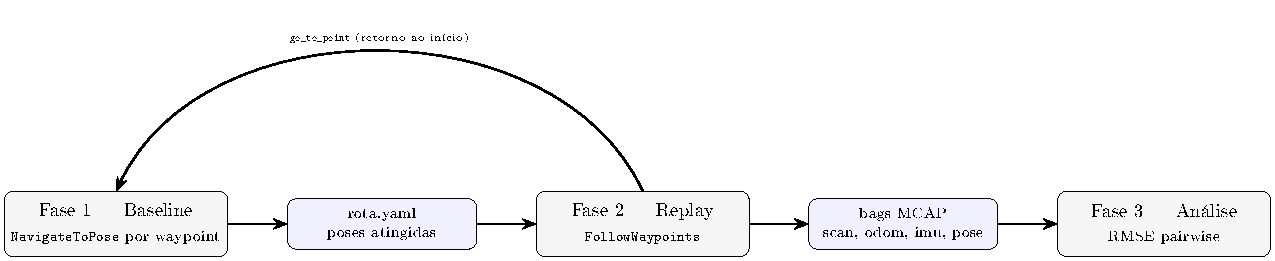
\includegraphics[width=\textwidth]{protocolo_record_replay.pdf}
\caption{Fluxo do protocolo record--replay: cada fase produz um artefato
explícito (rota YAML ou bag MCAP) consumido pela fase seguinte, permitindo
reexecução e auditoria independentes de cada etapa.}
\label{fig:protocolo_record_replay}
\end{figure}


\subsection{Fase 1 — Gravação do Baseline}

A gravação do baseline define a rota de referência. O pesquisador especifica um
conjunto de waypoints $\{w_1, w_2, \ldots, w_k\}$ no referencial do mapa SLAM.
O sistema ativa a coleta de sensores, aciona o \texttt{start\_\allowbreak record} no orquestrador
e comanda o robô via \texttt{NavigateToPose} sequencial para cada waypoint. Ao atingir
cada ponto, a pose real do robô é registrada no arquivo de rota YAML ---
não a pose solicitada, mas a pose efetivamente atingida conforme estimada pela
cadeia TF \texttt{map} $\to$ \texttt{base\_\allowbreak link}. Ao final, \texttt{stop\_\allowbreak record}
persiste o arquivo e \texttt{disable\_\allowbreak collection} fecha o bag.

A distinção entre waypoints solicitados e poses atingidas é essencial: o Nav2 para
quando a pose está dentro da tolerância configurada (tipicamente 25\,cm em posição
e 25\,cm em ângulo), não necessariamente no ponto exato. Gravar a pose atingida,
e não a solicitada, garante que o replay reproduza o que o robô \textit{fez},
não o que foi \textit{pedido} --- uma distinção relevante quando a análise de
repetibilidade compara execuções entre si.

\subsection{Fase 2 — Execuções de Replay}

As execuções de replay reproduzem a rota gravada. O orquestrador lê o arquivo
YAML do baseline e envia todas as poses como lista para o action
\texttt{FollowWaypoints}, que o Nav2 percorre de forma contínua. A diferença de
action em relação ao baseline (\texttt{NavigateToPose} sequencial vs.
\texttt{FollowWaypoints}) foi identificada como uma fonte de variação sistemática:
o segundo não para completamente em cada waypoint antes de planejar para o próximo,
produzindo trajetórias ligeiramente mais suaves e de menor duração. Para análises
de repetibilidade pura entre replays, essa diferença é irrelevante; para comparação
replay vs. baseline, deve ser documentada.

Antes de cada replay, o robô retorna ao ponto de partida via \texttt{go\_\allowbreak to\_\allowbreak point}
(opcional, configurável). Esse retorno é necessário quando o experimento exige que
o robô parta da mesma pose inicial em todas as execuções --- requisito fundamental
para isolamento de variáveis.

\subsection{Fase 3 — Análise Offline}

A análise é realizada offline sobre os bags coletados. Para cada bag, o script
\texttt{analyze\_\allowbreak runs.py} extrai a trajetória via odometria a 50\,Hz, filtra
saltos impossíveis (variações acima de 0,12\,m entre amostras a 50\,Hz),
e interpola todas as trajetórias para uma grade de tempo normalizada $\{t_1, t_2, \ldots, t_n\}$.
O RMSE pairwise é calculado conforme a Equação~\ref{eq:rmse_pairwise}.

Adicionalmente, o script gera: (i) CSV com as trajetórias interpoladas para
visualização externa; (ii) PNG de overlay das trajetórias com codificação visual
por execução; (iii) JSON de sumário com todas as métricas calculadas por par de
execuções.

\section{Métricas Adotadas}
\label{sec:metricas}

Quatro métricas quantificam a repetibilidade de navegação neste trabalho:

\begin{enumerate}
    \item \textbf{RMSE inter-replay}: RMSE pairwise entre as execuções de replay,
    excluindo o baseline. Mede a repetibilidade \textit{pura} do sistema de
    navegação quando operado nas mesmas condições.

    \item \textbf{RMSE replay vs. baseline}: RMSE entre cada replay e o baseline.
    Captura tanto a variabilidade de navegação quanto o eventual gap de estratégia
    entre os actions utilizados.

    \item \textbf{Erro de endpoint}: distância euclidiana entre as posições finais
    de dois percursos. Mede se o robô termina no mesmo lugar, independente do
    caminho percorrido.

    \item \textbf{Consistência temporal}: desvio padrão das durações entre execuções
    equivalentes. Um desvio pequeno indica que o controlador opera a velocidades
    estáveis e não encontra obstáculos que forcem replanejamentos.
\end{enumerate}

\subsection{Intervalo de Confiança para $N \geq 5$}
\label{sec:ic_estatistico}

Para cenários com cinco ou mais réplicas, o RMSE inter-replay é reportado como
média $\pm$ intervalo de confiança de 95\%, calculado via distribuição $t$ de
Student:

\begin{equation}
\text{IC}_{95\%} = \overline{\text{RMSE}} \pm t_{0{,}025,\, N-1} \cdot \frac{s}{\sqrt{N}}
\label{eq:ic_95}
\end{equation}

\noindent onde $\overline{\text{RMSE}}$ é a média das distâncias RMSE pairwise entre
replays, $s$ o desvio padrão amostral e $t_{0{,}025,\,N-1}$ o quantil da
distribuição $t$ de Student com $N-1$ graus de liberdade. A distribuição $t$,
em vez da normal, é usada por ser mais apropriada para amostras pequenas
($N < 30$), onde a variância populacional é desconhecida e estimada a partir
da própria amostra. Na campanha final desta dissertação, $N=10$ replays
fornecem uma estimativa descritiva mais estável da variabilidade observada; o
intervalo de confiança, contudo, deve ser interpretado no escopo estreito da
rota e do ambiente avaliados, não como generalização para outras configurações.

\section{Design dos Experimentos de Validação}
\label{sec:design_experimentos}

Um cenário controlado foi definido para validar o framework em simulação:

\textbf{Campanha dissertation\_clean01}: rota curta, aproximadamente retilínea,
executada no mundo \textit{warehouse} com TurtleBot4 Standard. A rota foi
escolhida para isolar a capacidade do framework de registrar, reproduzir e medir
uma trajetória sob condições rigorosamente controladas, antes de estender o
protocolo para percursos mais longos, curvas acentuadas ou obstáculos dinâmicos.

O protocolo executa uma baseline limpa e dez replays independentes. Diferentemente
das campanhas exploratórias iniciais, cada replay da campanha final é iniciado
após relançamento completo da simulação, da pilha Nav2 e dos nós de coleta. Essa
decisão metodológica garante que a pose inicial medida em \texttt{/\allowbreak odom}
seja praticamente a mesma em todas as execuções, evitando que o RMSE misture erro
de repetição da trajetória com diferença de condição inicial.


\section{Ambiente Experimental}
\label{sec:ambiente_hw}

A Tabela~\ref{tab:ambiente_hw} descreve o ambiente de hardware e software
utilizado em todas as execuções reportadas neste trabalho. A escolha de manter
todos os experimentos em um único ambiente controlado --- em vez de distribuí-los
entre máquinas com configurações distintas --- é deliberada: o objetivo desta
dissertação é isolar a variabilidade intrínseca ao pipeline de navegação
(SLAM, controlador, executor ROS~2), e não introduzir uma segunda fonte de
variação decorrente de diferenças de hardware entre execuções.

\begin{table}[H]
\centering
\caption{Ambiente experimental utilizado nas validações reportadas nesta dissertação.}
\label{tab:ambiente_hw}
\begin{tabular}{ll}
\toprule
\textbf{Componente} & \textbf{Especificação} \\
\midrule
Sistema operacional & Ubuntu 24.04 LTS \\
Middleware ROS & ROS~2 Jazzy Jalisco (instalação \textit{desktop}) \\
Simulador & Gazebo Harmonic \\
Pacote de simulação & \texttt{nav2\_\allowbreak minimal\_\allowbreak tb4\_\allowbreak sim} \\
Modelo de robô & TurtleBot4 Standard \\
Sensor LiDAR & RPLIDAR S2 (2D, 360°) \\
Sensor de imagem & Câmera OAK-D \\
Mundo de simulação & \textit{warehouse} (\texttt{nav2\_\allowbreak minimal\_\allowbreak tb4\_\allowbreak sim}) \\
Pilha de navegação & Navigation2 (Nav2), controlador MPPI \\
SLAM & SLAM Toolbox, modo síncrono \\
Formato de gravação & rosbag2 / MCAP \\
\bottomrule
\end{tabular}
\end{table}

\section{Fluxo de Execução do Protocolo}
\label{sec:fluxo_protocolo}

Na prática operacional, o protocolo descrito na Seção~\ref{sec:record_replay}
é executado como uma sequência ordenada de comandos, seja diretamente pela
linha de comando (via \texttt{experiment\_\allowbreak repeatability.py}), seja pela
interface web, que internamente dispara os mesmos comandos como um subprocesso
gerenciado pelo backend (Seção~\ref{sec:impl_backend_ponte}). O fluxo completo,
do ambiente limpo ao relatório de repetibilidade, compreende:

\begin{enumerate}
    \item \textbf{Inicialização da simulação}: subida do Gazebo, SLAM Toolbox
    (após um atraso de 8\,s para permitir que o \textit{bridge} de tópicos
    estabilize) e Nav2 (após 12\,s), aguardando a mensagem de log
    \texttt{All BT navigator servers are active} antes de prosseguir --- uma
    barreira de sincronização que evita o início prematuro de comandos de
    navegação contra um Nav2 ainda não pronto.

    \item \textbf{Inicialização dos nós de frota}: subida do
    \texttt{fleet\_\allowbreak orchestrator} e do \texttt{sensor\_\allowbreak collector}, aguardando as
    mensagens de prontidão \texttt{fleet\_\allowbreak orchestrator ready} e
    \texttt{sensor\_\allowbreak collector ready}.

    \item \textbf{Gravação do baseline}: definição de waypoints (via clique no
    mapa SLAM ao vivo, na interface web, ou via lista de coordenadas, na CLI) e
    execução do subcomando \texttt{record}, que invoca sequencialmente
    \texttt{start\_\allowbreak record}, uma série de \texttt{go\_\allowbreak to\_\allowbreak point} e
    \texttt{stop\_\allowbreak record} (Seção~\ref{sec:impl_servicos_exemplo}).

    \item \textbf{Execuções de replay}: repetição do subcomando \texttt{replay}
    $N$ vezes, cada uma invocando \texttt{play\_\allowbreak route} sobre a rota gravada no
    passo anterior, com retorno opcional ao ponto de partida
    (\texttt{--return-to-start}) entre execuções.

    \item \textbf{Exportação e análise offline}: ao final de cada execução, o
    \texttt{experiment\_\allowbreak repeatability.py} exporta um JSON de resumo por execução
    (via \texttt{--export}); posteriormente, \texttt{analyze\_\allowbreak runs.py} processa
    o conjunto de bags MCAP e produz o \texttt{summary.json} consolidado com as
    métricas de RMSE pairwise, o \texttt{trajectory\_\allowbreak overlay.png} e os CSVs por
    execução (Seção~\ref{sec:impl_pipeline}).
\end{enumerate}

Esse fluxo é o mesmo, independentemente de o pesquisador operar via terminal ou
via interface web: a Seção~\ref{sec:impl_backend_ponte} descreve como o backend
traduz a interação da UI para exatamente essa sequência de subcomandos, o que
garante que resultados obtidos por qualquer uma das duas vias sejam diretamente
comparáveis.

\section{Considerações Finais}
\label{sec:met_conclusao}

O protocolo record--replay formaliza o que muitos experimentos de robótica fazem
informalmente, adicionando precisão nos pontos críticos: a gravação da pose atingida
(não solicitada), o filtro de saltos impossíveis na odometria, a interpolação para
grade de tempo comum antes do cálculo de RMSE e o retorno explícito ao ponto de
partida entre execuções. O próximo capítulo descreve como esses procedimentos foram
implementados no código do framework.

\chapter{Implementação}
\label{chap:implementacao}

\section{Ambiente de Simulação}
\label{sec:simulacao}

Seguindo a prática estabelecida de validar algoritmos de navegação em simulação
ROS~+~Gazebo antes de sua implantação no robô físico \cite{takaya2016}, o
ambiente de simulação utiliza o Gazebo Harmonic --- versão de suporte estendido
pareada com o ROS~2 Jazzy --- e o modelo TurtleBot4 Standard com RPLIDAR S2 (LiDAR
2D de 360°) e câmera OAK-D. O mundo \textit{warehouse} disponível no pacote
\texttt{nav2\_\allowbreak minimal\_\allowbreak tb4\_\allowbreak sim} representa um armazém industrial com prateleiras,
barreiras e espaços abertos, oferecendo diversidade de geometria para testar o SLAM
em diferentes condições de observabilidade.

A escolha do \texttt{nav2\_\allowbreak minimal\_\allowbreak tb4\_\allowbreak sim} em detrimento do
\texttt{turtlebot4\_\allowbreak gz\_\allowbreak bringup} resultou de problemas de compatibilidade entre os
plugins \texttt{irobot\_\allowbreak create\_\allowbreak gz\_\allowbreak plugins} --- projetados para Ignition Fortress ---
e o Gazebo Harmonic, que renomeou a API de mensagens de \texttt{ignition.msgs} para
\texttt{gz.msgs}. A versão minimal contorna esse problema utilizando o plugin de
DiffDrive nativo do Gazebo Harmonic com bridges corretos, incluindo o topic
\texttt{cmd\_\allowbreak vel} como \texttt{geometry\_\allowbreak msgs/\allowbreak msg/\allowbreak Twist} (não \texttt{TwistStamped}).
Essa distinção exigiu que os parâmetros de navegação do Nav2 fossem gerados em tempo
de launch com \texttt{enable\_\allowbreak stamped\_\allowbreak cmd\_\allowbreak vel: false} em todos os onze nós afetados,
via leitura e patch programático do arquivo \texttt{nav2.yaml} padrão.

\section{O Orquestrador em Detalhe}
\label{sec:impl_orquestrador}

O orquestrador (\texttt{fleet\_\allowbreak orchestrator}) é implementado como um nó ROS~2 em Python
com \texttt{MultiThreadedExecutor}. A estrutura de estado por robô, \texttt{RobotRuntime},
mantém seis campos: \texttt{nav\_\allowbreak state}, \texttt{is\_\allowbreak recording}, \texttt{is\_\allowbreak navigating},
\texttt{route\_\allowbreak poses}, \texttt{last\_\allowbreak saved} e \texttt{pending\_\allowbreak goal\_\allowbreak pose}. Este último
é o mais crítico para a gravação: ao receber o callback de resultado do action Nav2,
se o status for \texttt{STATUS\_\allowbreak SUCCEEDED} e o robô estiver em modo de gravação,
a pose enviada como meta é imediatamente appendada à lista de rotas --- pois a pose
real confirmada pelo Nav2 é a melhor estimativa disponível da posição atingida.

A lógica de gravação baseada em polling de TF (\texttt{\_\allowbreak record\_\allowbreak tick}) funciona em
paralelo para ambientes onde o Nav2 não reporta SUCCEEDED (e.g., quando o controlador
para dentro da tolerância antes de publicar o callback). O tick a 5\,Hz consulta a
cadeia TF e adiciona a pose ao buffer se o robô deslocou ao menos 10\,cm ou girou
mais de 5° desde a última amostra, evitando redundância em trechos estacionários.


\subsection{Exemplo: os Serviços \texttt{start\_\allowbreak record} e \texttt{stop\_\allowbreak record}}
\label{sec:impl_servicos_exemplo}

Para tornar concreta a discussão anterior, o Código~\ref{lst:start_stop_record}
reproduz, tal como publicado no repositório público do projeto, os \textit{callbacks}
que implementam o início e o fim de uma gravação de rota. Note-se a rejeição explícita
de requisições inconsistentes com o estado corrente do robô (\texttt{ALREADY\_\allowbreak NAVIGATING})
e a limpeza do buffer de poses e do último ponto salvo (\texttt{last\_\allowbreak saved = None}) a
cada novo início de gravação --- sem essa limpeza, uma segunda gravação herdaria pontos
da anterior, corrompendo silenciosamente o arquivo de rota resultante.

\begin{lstlisting}[style=pycode, caption={Callbacks \texttt{\_\allowbreak cb\_\allowbreak start\_\allowbreak record} e \texttt{\_\allowbreak cb\_\allowbreak stop\_\allowbreak record} (\texttt{fleet\_\allowbreak orchestrator/\allowbreak main.py}).}, label={lst:start_stop_record}]
def _cb_start_record(self, req, resp):
    rid = req.robot_id
    if not self._known_robot(rid):
        resp.success = False
        resp.message = f"Unknown robot {rid!r}"
        resp.error_code = "UNKNOWN_ROBOT"
        return resp
    st = self._state[rid]
    if st.is_navigating:
        resp.success = False
        resp.message = "Cannot start recording while navigating"
        resp.error_code = "ALREADY_NAVIGATING"
        return resp
    st.route_poses.clear()
    st.last_saved = None
    st.is_recording = True
    st.nav_state = "recording"
    st.current_route = req.route_name
    st.last_error = ""
    resp.success = True
    resp.message = "Recording started"
    resp.error_code = ""
    return resp

def _cb_stop_record(self, req, resp):
    rid = req.robot_id
    if not self._known_robot(rid):
        resp.success = False
        resp.message = f"Unknown robot {rid!r}"
        resp.error_code = "UNKNOWN_ROBOT"
        return resp
    st = self._state[rid]
    route_name = st.current_route
    st.is_recording = False
    n = len(st.route_poses)
    if n == 0:
        st.nav_state = "idle"
        st.current_route = ""
        resp.success = True
        resp.message = "Route length: 0"
        resp.error_code = ""
        return resp
    path = self._save_route_yaml(rid, route_name, st.route_poses)
    st.route_poses.clear()
    st.last_saved = None
    st.nav_state = "idle"
    st.current_route = ""
    resp.success = True
    resp.message = f"Saved {n} poses to {path}"
    resp.error_code = ""
    return resp
\end{lstlisting}

Um segundo aspecto relevante do orquestrador é a separação entre os papéis
experimentais e a permissão de movimento, aplicada em \texttt{\_\allowbreak cb\_\allowbreak play\_\allowbreak route}
e \texttt{\_\allowbreak cb\_\allowbreak go\_\allowbreak to\_\allowbreak point} por meio do método \texttt{\_\allowbreak motion\_\allowbreak allowed},
que consulta o mapa de papéis carregado de \texttt{roles.yaml} e retorna
\texttt{False} para qualquer robô que não seja \texttt{MUUT}. Requisições de
movimento para um FUUT recebem o código de erro \texttt{ROLE\_\allowbreak NOT\_\allowbreak ALLOWED}
antes mesmo de qualquer tentativa de contato com o action server do Nav2,
evitando gastar o \textit{timeout} de \texttt{wait\_\allowbreak for\_\allowbreak server} em uma
requisição que já se sabe inválida por construção.

\subsection{A Ponte REST--ROS~2 no Backend}
\label{sec:impl_backend_ponte}

O backend não utiliza um cliente ROS~2 nativo para encaminhar comandos de
serviço vindos da interface web: em vez disso, cada endpoint HTTP dispara
um processo \texttt{ros2 service call} via \texttt{subprocess}, como mostra
o Código~\ref{lst:backend_bridge}. A justificativa para essa escolha, aparentemente
pouco ortodoxa, está detalhada na Seção~\ref{sec:backend_web}: evitar que o
processo do backend precise ele mesmo inicializar um nó \texttt{rclpy} completo
só para chamadas pontuais de serviço, mantendo essa inicialização (via
\texttt{rclpy.init()} em uma \textit{thread} dedicada) restrita à publicação
contínua de status, mapa e pose, que de fato exige um nó ROS~2 residente.

\begin{lstlisting}[style=pycode, caption={Função \texttt{\_\allowbreak run\_\allowbreak ros2\_\allowbreak service}, usada por todos os endpoints \texttt{/\allowbreak api/\allowbreak *} que encaminham comandos ao orquestrador (\texttt{backend/\allowbreak main.py}).}, label={lst:backend_bridge}]
def _run_ros2_service(srv, srv_type, request_json, timeout=10):
    cmd = (
        f"source /opt/ros/jazzy/setup.bash 2>/dev/null; "
        f"source {ROS_WS}/install/setup.bash 2>/dev/null; "
        f"ros2 service call {srv} {srv_type} '{request_json}'"
    )
    try:
        r = subprocess.run(
            ["bash", "-c", cmd],
            env=_ros_env(),
            capture_output=True,
            text=True,
            timeout=timeout,
            cwd=ROS_WS,
        )
        out = (r.stdout or "").strip() + (r.stderr or "").strip()
        if r.returncode != 0:
            return False, out or "ros2 service call failed"
        return True, out
    except subprocess.TimeoutExpired:
        return False, "timeout"
    except Exception as e:
        return False, str(e)
\end{lstlisting}

Essa abordagem tem um custo mensurável: cada chamada paga o overhead de
inicializar um processo \texttt{ros2 service call} (tipicamente
50--150\,ms na máquina de desenvolvimento), o que a torna inadequada para
comandos de alta frequência, mas aceitável para o padrão de uso da interface
--- cliques esparsos do pesquisador, não um laço de controle. O preço em
latência é trocado por uma superfície de acoplamento mínima entre o backend
e o \textit{workspace} ROS~2: o backend só precisa saber o nome e o tipo do
serviço, nunca importar diretamente os módulos gerados de \texttt{fleet\_\allowbreak msgs}
para essas chamadas específicas.

\section{Pipeline de Coleta e Análise}
\label{sec:impl_pipeline}

O script \texttt{experiment\_\allowbreak repeatability.py} implementa o protocolo descrito no
Capítulo~\ref{chap:metodologia} como uma sequência de chamadas a serviços ROS~2.
Sua estrutura em dois subcomandos (\texttt{record} e \texttt{replay}) permite compor
qualquer protocolo experimental a partir de blocos elementares, seja pela linha de
comando ou pela interface web.

A análise offline em \texttt{analyze\_\allowbreak runs.py} lê os bags via \texttt{rosbag2\_\allowbreak py},
desserializando diretamente as mensagens de tipos conhecidos
(\texttt{nav\_\allowbreak msgs/\allowbreak Odometry}, \texttt{geometry\_\allowbreak msgs/\allowbreak PoseWithCovarianceStamped})
a partir do formato CDR armazenado no MCAP. A versão do script utilizada na
campanha final desta dissertação calcula o RMSE pairwise após reamostragem em
tempo normalizado: cada trajetória é projetada para uma grade comum no intervalo
$[0,1]$, e as coordenadas $x$ e $y$ são interpoladas nessa grade antes do cálculo
do erro quadrático médio. Essa escolha evita associar pontos apenas pelo índice
da amostra, o que poderia introduzir artefatos quando duas execuções percorrem
a mesma rota com pequenas diferenças de velocidade.

Para fins de auditoria, o próprio \texttt{summary.json} produzido pela análise
registra o modo de reamostragem usado. Na campanha final
\texttt{dissertation\_\allowbreak clean01\_\allowbreak final\_\allowbreak manual}, o campo
\texttt{resampling.mode} indica \texttt{time}, com 100 amostras na grade
normalizada.


\subsection{Reamostragem e RMSE: o Código que Sustenta a Métrica}
\label{sec:impl_rmse_codigo}

O Código~\ref{lst:rmse_impl} reproduz as funções centrais de reamostragem e
cálculo de RMSE em \texttt{analyze\_\allowbreak runs.py}. A função
\texttt{\_\allowbreak normalised\_\allowbreak time\_\allowbreak grid} converte o vetor temporal de cada bag
para o intervalo $[0,1]$; em seguida, \texttt{numpy.interp} calcula posições
homólogas na mesma grade normalizada. A implementação por índice permanece
disponível como opção de compatibilidade (\texttt{--resample-mode index}), mas
não foi usada na campanha final reportada no Capítulo~\ref{chap:resultados}.

\begin{lstlisting}[style=pycode, caption={Reamostragem temporal normalizada e RMSE pairwise (\texttt{scripts/\allowbreak analyze\_\allowbreak runs.py}).}, label={lst:rmse_impl}]
def _normalised_time_grid(t):
    if len(t) < 2:
        return np.zeros(len(t), dtype=np.float64)
    duration = float(t[-1] - t[0])
    if duration <= 1e-9:
        return np.linspace(0.0, 1.0, len(t), dtype=np.float64)
    return (t - t[0]) / duration

def _resample_xy_by_time(t, xy, samples):
    if len(xy) < 2 or samples < 2:
        return xy
    tn = _normalised_time_grid(t)
    unique_t, unique_idx = np.unique(tn, return_index=True)
    unique_xy = xy[unique_idx]
    grid = np.linspace(0.0, 1.0, samples, dtype=np.float64)
    return np.column_stack([
        np.interp(grid, unique_t, unique_xy[:, 0]),
        np.interp(grid, unique_t, unique_xy[:, 1]),
    ])

def _rmse(a, b):
    return float(np.sqrt(np.mean(np.sum((a - b) ** 2, axis=1))))
\end{lstlisting}

A consequência prática dessa escolha é que duas trajetórias percorridas em
velocidades ligeiramente distintas continuam comparáveis, pois os pontos
homólogos representam a mesma fração normalizada do percurso temporal de cada
execução. Essa formulação não elimina todas as ameaças à validade --- diferenças
muito grandes de duração ainda podem indicar que as execuções não são
experimentalmente equivalentes ---, mas reduz o artefato geométrico introduzido
pela reamostragem puramente por índice.

\section{Interface Web}
\label{sec:impl_web}

A interface web é uma aplicação React com backend FastAPI. O mapa SLAM é renderizado
em um canvas HTML5 com coordenadas alinhadas ao sistema de referência ROS: a origem
do canvas corresponde ao canto inferior esquerdo do mapa, e o eixo Y é invertido
(positivo para cima em ROS, negativo no canvas). A conversão utiliza os metadados
do \texttt{OccupancyGrid} \cite{elfes1989} (\texttt{resolution}, \texttt{origin\_\allowbreak x}, \texttt{origin\_\allowbreak y})
publicados pelo SLAM Toolbox.

O mapa pré-construído do \textit{warehouse} (\texttt{warehouse.pgm} +
\texttt{warehouse.yaml}) é utilizado como fundo estático com alinhamento perfeito:
como ambos o mapa SLAM ao vivo e o PGM utilizam o mesmo sistema de coordenadas
do mundo Gazebo, a sobreposição é pixel-a-pixel. O pesquisador vê paredes, prateleiras
e o robô em tempo real, podendo clicar para definir waypoints diretamente na planta.

\section{Considerações Finais}
\label{sec:impl_conclusao}

As decisões de implementação descritas neste capítulo --- o patch runtime do
\texttt{nav2.yaml}, o \texttt{MultiThreadedExecutor} para evitar deadlocks, a
desserialização CDR sem tipo registrado, a conversão de coordenadas canvas--mundo
--- resultaram de problemas concretos encontrados durante o desenvolvimento.
Cada uma representa uma contribuição de engenharia que outros grupos de pesquisa
que adotarem o framework não precisarão replicar. O próximo capítulo apresenta
o arranjo de avaliação que valida o sistema resultante.

\chapter{Avaliação}
\label{chap:avaliacao}

\section{Arranjo Experimental}
\label{sec:arranjo}

A avaliação do framework foi conduzida em simulação Gazebo Harmonic com um robô
TurtleBot4 Standard no mundo \textit{warehouse}. O ambiente de simulação garante
condições perfeitamente repetíveis dentro do mesmo laboratório --- sem variação de iluminação, temperatura
ou tráfego de outros agentes --- o que permite isolar a variabilidade introduzida
pelos algoritmos de navegação e SLAM da variabilidade ambiental. Experimentos em
hardware real, com sua camada adicional de incerteza, constituem trabalho futuro.

A configuração da pilha de software é:

\begin{itemize}
    \item \textbf{Sistema operacional}: Ubuntu 24.04 LTS (Noble Numbat)
    \item \textbf{ROS~2}: Jazzy Jalisco (LTS)
    \item \textbf{Simulador}: Gazebo Harmonic 8.x
    \item \textbf{Navegação}: Nav2 (pacotes \texttt{ros-jazzy-nav2-*})
    \item \textbf{SLAM}: SLAM Toolbox (modo síncrono)
    \item \textbf{Plataforma}: TurtleBot4 Standard (via \texttt{nav2\_\allowbreak minimal\_\allowbreak tb4\_\allowbreak sim})
\end{itemize}

\section{Questões de Avaliação}
\label{sec:questoes}

Três questões orientam a avaliação:

\begin{description}
    \item[QA1] O framework consegue executar o protocolo record--replay de forma
    automática e sem intervenção manual entre as fases?

    \item[QA2] Qual é o RMSE inter-replay observado em uma campanha controlada
    com dez execuções independentes iniciadas a partir do mesmo estado? Os
    valores ficam abaixo da tolerância padrão do Nav2 (25\,cm)?

    \item[QA3] A consistência temporal entre execuções equivalentes é suficiente
    para justificar comparações de trajetória baseadas em reamostragem temporal
    normalizada?

    \item[QA4] A repetibilidade observada sob o protocolo controlado (QA2, QA3)
    se mantém quando as execuções ocorrem fora desse regime controlado --- sem
    a mesma ação de navegação, pose inicial fixa ou retorno explícito ao ponto
    de partida entre réplicas? Esta questão foi adicionada durante a execução
    do trabalho, motivada pela disponibilidade de três conjuntos de dados
    exploratórios adicionais no repositório do projeto
    (Seção~\ref{sec:res_exp_complementares}), e por isso é tratada como
    evidência diagnóstica, não como conclusão causal principal.
\end{description}

QA1 corresponde à hipótese H1; QA2 e QA3, em conjunto, correspondem a H2; QA4
corresponde a H3 (Seção~\ref{sec:perguntas_pesquisa}). Não há uma questão de
avaliação dedicada a H4 (custo de engenharia): como discutido na
Seção~\ref{sec:retomada_pp}, essa hipótese é avaliada apenas qualitativamente,
não por um critério mensurável como QA1--QA4.

\section{Procedimento}
\label{sec:procedimento}

Para a campanha final de avaliação, o procedimento é:

\begin{enumerate}
    \item Iniciar uma sessão limpa de simulação Gazebo Harmonic com TurtleBot4
    Standard.
    \item Aguardar ativação completa do Nav2, SLAM Toolbox, sensores e serviços
    do orquestrador.
    \item Gravar uma baseline limpa (\texttt{dissertation\_\allowbreak clean01}) por
    navegação sequencial pelos waypoints definidos para a rota curta de validação.
    \item Armazenar a rota resultante em YAML e o bag MCAP da baseline.
    \item Executar dez replays independentes da rota gravada.
    \item Antes de cada replay, relançar completamente a simulação, a pilha Nav2,
    o orquestrador e o coletor de sensores, garantindo que a odometria inicie no
    mesmo estado em todas as execuções.
    \item Em cada replay, aguardar explicitamente o mapa do SLAM, a estabilização
    do costmap e o estado \texttt{active} dos nós lifecycle do Nav2 antes de enviar
    a rota.
    \item Coletar \texttt{/\allowbreak scan}, \texttt{/\allowbreak odom}, \texttt{/\allowbreak imu} e
    \texttt{/\allowbreak pose} em formato MCAP.
    \item Executar \texttt{analyze\_\allowbreak runs.py} sobre os dez bags, usando
    \texttt{/\allowbreak odom} como fonte da trajetória e reamostragem temporal
    normalizada.
\end{enumerate}

\section{Critérios de Validação}
\label{sec:criterios}

O framework é considerado válido se:

\begin{enumerate}
    \item O protocolo completo (baseline, dez replays e análise) for executado
    com orquestração automática das fases principais (\textbf{QA1}).

    \item Todos os replays válidos começarem do mesmo estado inicial medido em
    \texttt{/\allowbreak odom}.

    \item O RMSE médio e máximo contra a execução de referência forem inferiores
    a 25\,cm (\textbf{QA2}).

    \item O erro final médio e máximo permanecerem inferiores a 25\,cm.

    \item O desvio de duração entre execuções equivalentes for inferior a 10\%
    da duração média (\textbf{QA3}).
\end{enumerate}

O limiar de 10\% acima é usado como critério mínimo de aceitação para QA3. Ele
não significa que durações diferentes sejam desejáveis, apenas que variações
abaixo desse patamar são pequenas o suficiente para sustentar a comparação por
tempo normalizado no cenário controlado. A campanha final ficou abaixo desse
limiar, como apresentado na Seção~\ref{sec:res_qa3}.

\section{Ameaças à Validade}
\label{sec:ameacas}

Seguindo a prática de reportar ameaças à validade em pesquisa empírica de
Engenharia de Software \cite{amigoni2010}, e em resposta ao diagnóstico de
rigor metodológico limitado --- comparação estatística fraca, baixa
disponibilidade de artefatos --- identificado em experimentos de robótica
autônoma publicados \cite{amigoni2014}, esta seção examina os limites da
avaliação nas quatro dimensões clássicas, na linha do que
\citeonline{bonsignorio2015} defendem como pesquisa em robótica replicável e
mensurável.

\textbf{Validade de construto.} O RMSE foi calculado a partir do tópico
\texttt{/\allowbreak odom}, não de um sistema de captura de movimento externo. Tanto a
odometria quanto a pose estimada pelo SLAM são gravadas nos bags, o que permite
comparações cruzadas futuras com uma referência externa. Em simulação, a
odometria é gerada pelo plugin DiffDrive do Gazebo e, portanto, é menos ruidosa
que encoders físicos reais; em robôs físicos, slip de roda e condições do piso
exigiriam uma referência externa ou comparação direta com a pose do SLAM.

Um risco de validade de construto foi identificado e corrigido durante o
desenvolvimento: o modo automático de detecção de tópico do
\texttt{analyze\_\allowbreak runs.py} originalmente só reconhecia um tópico chamado
literalmente \texttt{amcl\_\allowbreak pose}; como este trabalho usa SLAM Toolbox, e não
AMCL, esse tópico nunca existe, e a análise recaía silenciosamente em
\texttt{/\allowbreak odom} mesmo quando a pose corrigida do SLAM
(\texttt{/\allowbreak pose}) também havia sido gravada no mesmo bag. Esse
comportamento poderia inflar artificialmente o RMSE em rotas mais longas ou
demoradas, já que a odometria bruta deriva continuamente enquanto a pose do
SLAM é corrigida pelo casamento de \textit{scans} contra o mapa. O modo
automático foi corrigido para priorizar, nessa ordem, \texttt{amcl\_\allowbreak pose}
$>$ \texttt{pose} (SLAM Toolbox) $>$ \texttt{odom}, escolhendo a primeira opção
com mensagens de fato gravadas; a seleção também pode ser forçada
explicitamente. Análises realizadas antes dessa correção que tenham caído no
\textit{fallback} de \texttt{/\allowbreak odom} deveriam, a rigor, ser
reconsideradas caso a pose do SLAM também estivesse disponível no mesmo bag.

Uma segunda fonte de viés de construto, evidenciada em execuções exploratórias
reais (Seção~\ref{sec:res_exp_complementares}), é que a fase de gravação e a
fase de replay não navegam pelo mesmo mecanismo: \texttt{record} envia uma
sequência de comandos \texttt{go\_\allowbreak to\_\allowbreak point}, um objetivo Nav2 de
cada vez, com o robô assentando em cada waypoint antes de o próximo ser
enviado; \texttt{replay} envia uma única \texttt{play\_\allowbreak route}, percorrendo a
rota inteira como navegação contínua. Em uma campanha exploratória com essa
configuração (rota de quatro waypoints, $N=3$ replays), o RMSE par-a-par entre
replays foi da ordem de 0,02\,m, contra cerca de 0,14\,m entre a baseline e
cada replay, com a baseline durando cerca de 2,5$\times$ menos que os replays
--- diferença explicada quase inteiramente pelo mecanismo de navegação
distinto, não por falta de repetibilidade do robô. Por esse motivo, o RMSE
calculado entre replays entre si (que compartilham o mesmo mecanismo de
navegação) é a métrica mais fiel à repetibilidade que este trabalho pretende
medir --- seguindo a mesma lógica metodológica adotada por
\citeonline{maset2022} para repetibilidade em mapeamento 3D, de comparar
execuções nominalmente idênticas diretamente entre si em vez de cada uma
isoladamente contra um único valor de referência; comparações contra a
gravação baseline, que usa um mecanismo de
navegação distinto, misturam essa diferença de implementação com
repetibilidade real e devem ser interpretadas com essa ressalva.

\textbf{Validade interna.} Campanhas preliminares sem reinicialização do estado
entre replays produziram trajetórias cujos pontos iniciais coincidiam com os
pontos finais da execução anterior, misturando erro de repetição com erro de
inicialização. Por esse motivo, tais campanhas foram tratadas como diagnósticas,
e não como resultado final. A campanha reportada nesta dissertação corrige essa
ameaça ao relançar a simulação e os nós de navegação/coleta antes de cada replay,
fazendo com que os dez bags analisados comecem praticamente no mesmo ponto em
\texttt{/\allowbreak odom}. Ainda assim, fatores como variação interna do controlador
local, estado do SLAM e estabilização do costmap continuam sendo possíveis fontes
de variabilidade residual. Em particular, o controlador local usado
(\texttt{nav2\_\allowbreak mppi\_\allowbreak controller}, algoritmo MPPI --- \textit{Model
Predictive Path Integral} \cite{williams2016}) é estocástico por projeto: a
cada ciclo de controle
(20\,Hz), com \texttt{regenerate\_\allowbreak noises: true}, ruído gaussiano é
reamostrado sobre a trajetória candidata. Ou seja, duas execuções da mesma
rota, no mesmo robô e no mesmo ambiente, divergem parcialmente apenas pela
amostragem aleatória do controlador --- isso não é falha de repetibilidade do
sistema avaliado, é ruído esperado e não-eliminável do método de controle
escolhido (a menos que se troque por um controlador determinístico, como DWB
ou Regulated Pure Pursuit, alternativa não avaliada nesta dissertação).
Adicionalmente, o critério de chegada do Nav2 (\texttt{general\_\allowbreak goal\_\allowbreak
checker}) aceita até 0,25\,m de erro de posição e 0,25\,rad (aproximadamente
14°) de erro angular; desvios de endpoint dentro dessa faixa refletem o
comportamento configurado do Nav2, não necessariamente imprecisão do
framework de medição.

\textbf{Validade externa.} A validação usa simulação com TurtleBot4 em um único
ambiente (\textit{warehouse}). Hardware real introduziria slip de roda, ruído de
sensores, erro de calibração e efeitos de superfície não modelados pelo Gazebo.
Ainda assim, a arquitetura foi projetada para minimizar dependências
específicas de plataforma: o orquestrador depende de actions, tópicos e
transforms padrão do ROS~2/Nav2 --- não de interfaces proprietárias do
TurtleBot4 --- o que favorece, em princípio, a generalização para outras
plataformas com a mesma pilha de navegação. Essa generalização não foi
testada empiricamente nesta dissertação com nenhuma outra plataforma.

\textbf{Validade de conclusão.} A campanha final controlada utiliza $N=10$
replays, o que melhora substancialmente a estimativa de variabilidade em relação
às execuções exploratórias iniciais. Ainda assim, os resultados permanecem
restritos a um único cenário, uma única rota curta, um único robô simulado e uma
única configuração de Nav2. Portanto, embora a campanha seja suficiente para
demonstrar a capacidade do framework de automatizar e medir repetibilidade sob
condições controladas, ela não deve ser interpretada como caracterização
estatística geral do comportamento do TurtleBot4, do Nav2 ou do SLAM Toolbox em
qualquer ambiente. A opção é, portanto, pela profundidade de análise por
execução em detrimento da amplitude de cenários: ao contrário de validações
agregadas de longa distância como o Marathon~2 \cite{macenski2020marathon},
que percorrem dezenas de quilômetros em ambientes variados mas reportam
critérios agregados (distância total, intervenções humanas) sem análise de
consistência entre execuções individuais, esta dissertação restringe o
escopo ambiental para poder medir exatamente essa consistência.

\section{Considerações Finais}
\label{sec:aval_conclusao}

O arranjo de avaliação foi concebido para responder às questões de forma direta e
verificável. A escolha por simulação sacrifica o realismo físico em favor do controle
experimental --- uma troca razoável para uma primeira validação de framework,
onde o objetivo é demonstrar que o sistema funciona como projetado, não que o
hardware físico se comporta de determinada forma. Os resultados são apresentados
no capítulo seguinte.

\chapter{Resultados}
\label{chap:resultados}

\section{QA1 — Automatização do Protocolo}
\label{sec:res_qa1}

O protocolo record--replay foi executado de forma automática em duas etapas.
Primeiro, uma baseline limpa foi gravada na rota
\texttt{dissertation\_\allowbreak clean01}, gerando o arquivo YAML de rota e um
bag MCAP com \texttt{/\allowbreak scan}, \texttt{/\allowbreak odom},
\texttt{/\allowbreak imu} e \texttt{/\allowbreak pose}. Em seguida, foram
executados dez replays independentes dessa rota. Para cada replay, um script de
campanha relançou completamente a simulação, a pilha Nav2, o orquestrador e o
coletor de dados, aguardou a ativação dos nós lifecycle do Nav2 e então iniciou
a coleta e a reprodução da rota.

A campanha final foi concluída com dez replays válidos, todos com
\texttt{success: true}. Os artefatos principais foram armazenados em
\texttt{fleet\_\allowbreak ws/\allowbreak runs/\allowbreak dissertation\_\allowbreak clean01\_\allowbreak final\_\allowbreak manual/},
incluindo o manifesto da campanha, os exports individuais de cada replay, os
bags MCAP, os CSVs de trajetória, o gráfico de sobreposição das trajetórias e o
arquivo \texttt{summary.json} consolidado.

\section{QA2 — RMSE de Repetibilidade}
\label{sec:res_qa2}

A Tabela~\ref{tab:campanha_final} apresenta as métricas por replay da campanha
final. O primeiro replay é usado como execução de referência; por isso, seu RMSE
e erro final contra a referência são iguais a zero e não entram no cálculo das
médias de erro.

\begin{table}[H]
\centering
\caption{Campanha final controlada: duração, comprimento, RMSE e erro final por replay.}
\label{tab:campanha_final}
\footnotesize
\begin{tabular}{lrrrr}
\toprule
\textbf{Execução} & \textbf{Duração (s)} & \textbf{Comprimento (m)} & \textbf{RMSE vs.\ ref. (cm)} & \textbf{Erro final (cm)} \\
\midrule
Replay 01 & 17,96 & 0,840 & 0,00 & 0,00 \\
Replay 02 & 17,64 & 0,807 & 2,57 & 3,26 \\
Replay 03 & 18,11 & 0,823 & 2,01 & 1,64 \\
Replay 04 & 17,57 & 0,824 & 2,58 & 1,56 \\
Replay 05 & 17,42 & 0,825 & 3,77 & 1,47 \\
Replay 06 & 17,32 & 0,847 & 4,58 & 0,67 \\
Replay 07 & 17,28 & 0,826 & 4,19 & 1,36 \\
Replay 08 & 17,32 & 0,825 & 4,76 & 1,50 \\
Replay 09 & 17,71 & 0,830 & 1,65 & 1,00 \\
Replay 10 & 16,78 & 0,817 & 4,08 & 2,26 \\
\bottomrule
\end{tabular}
\end{table}

Considerando os nove replays comparados à referência, o RMSE médio foi de
3,35\,cm, com desvio-padrão de 1,10\,cm. O menor RMSE observado foi de
1,65\,cm e o maior foi de 4,76\,cm. Todos os valores ficaram substancialmente
abaixo da tolerância padrão de objetivo do Nav2 de 25\,cm.

O resultado é metodologicamente mais forte que as campanhas preliminares porque
os pontos iniciais foram controlados. No \texttt{summary.json}, todos os dez
replays apresentam \texttt{start\_\allowbreak xy} praticamente igual a $(0,0)$,
com desvio máximo da ordem de $10^{-18}$\,m em relação ao primeiro replay.
Portanto, o RMSE medido não está misturando diferenças progressivas de pose
inicial com erro de repetição da trajetória.

A distância final em relação ao \texttt{replay\_\allowbreak 01} também permaneceu
baixa: o erro final médio foi de 1,64\,cm, com máximo de 3,26\,cm. Isso indica
que, além de seguir trajetórias semelhantes ao longo do percurso, o robô terminou
consistentemente em posições próximas sob o protocolo controlado.

\section{QA3 — Consistência Temporal}
\label{sec:res_qa3}

A duração média dos dez replays foi de 17,51\,s, com desvio-padrão de
0,36\,s. O comprimento médio estimado por \texttt{/\allowbreak odom} foi de
0,826\,m, com desvio-padrão de 0,010\,m. A variação temporal observada é
pequena para o objetivo da análise e compatível com o uso de reamostragem em
tempo normalizado.

Esses valores mostram que as execuções foram não apenas espacialmente próximas,
mas também temporalmente consistentes. A combinação de baixo RMSE, baixo erro
final e baixa dispersão de duração sustenta a interpretação de que o framework
reproduziu a rota de forma repetível sob condições controladas.

\section{Integridade dos Bags de Sensores}
\label{sec:res_bags}

Os dez bags da campanha final contêm os tópicos planejados:
\texttt{/\allowbreak scan}, \texttt{/\allowbreak odom}, \texttt{/\allowbreak imu}
e \texttt{/\allowbreak pose}. A Tabela~\ref{tab:sensor_bags} resume as
contagens médias de mensagens e as frequências efetivas estimadas por tópico.

\begin{table}[H]
\centering
\caption{Frequências efetivas médias de coleta de sensores na campanha final.}
\label{tab:sensor_bags}
\begin{tabular}{lrrr}
\toprule
\textbf{Tópico} & \textbf{Msgs/exec. média} & \textbf{Faixa de msgs} & \textbf{Freq. efetiva média (Hz)} \\
\midrule
\texttt{/\allowbreak scan} & 175,4 & 168--181 & 10,0 \\
\texttt{/\allowbreak odom} & 487,4 & 467--504 & 27,8 \\
\texttt{/\allowbreak imu}  & 3504,7 & 3364--3630 & 199,7 \\
\texttt{/\allowbreak pose} & 4,9 & 4--7 & 0,3 \\
\bottomrule
\end{tabular}
\end{table}

A trajetória principal da análise foi extraída de \texttt{/\allowbreak odom};
\texttt{/\allowbreak pose} foi preservado como dado auxiliar. A presença
consistente desses tópicos nos dez bags confirma que a coleta em MCAP permaneceu
operacional mesmo com o relançamento completo da simulação entre replays.

\section{Experimentos Complementares: Variabilidade Fora do Protocolo Controlado}
\label{sec:res_exp_complementares}

Antes da campanha final controlada, foram executadas campanhas exploratórias nas
quais os replays não eram reinicializados a partir do mesmo estado. Esses dados
foram úteis para diagnosticar uma ameaça metodológica: o início de uma execução
podia coincidir com o fim da anterior, especialmente quando
\texttt{return\_\allowbreak to\_\allowbreak start=false}. Nesses casos, a abertura
entre curvas não pode ser interpretada diretamente como erro puro de
repetibilidade, pois mistura repetição da trajetória com variação de pose inicial.

Um exemplo desse problema apareceu em campanhas nas quais o \texttt{start\_\allowbreak xy}
de um replay era praticamente igual ao \texttt{end\_\allowbreak xy} do replay
anterior. O efeito visual era uma separação progressiva entre trajetórias, mas
essa separação não media apenas a variabilidade do controlador ou do SLAM; media
também a consequência de iniciar cada nova execução a partir de uma pose diferente.

Por essa razão, os resultados exploratórios são mantidos como evidência
diagnóstica e motivação do protocolo final, mas não substituem a campanha
\texttt{dissertation\_\allowbreak clean01\_\allowbreak final\_\allowbreak manual}, na qual
o estado inicial foi efetivamente controlado. O principal valor desses dados é
mostrar empiricamente que a infraestrutura de coleta não basta: para que o RMSE
seja interpretável como repetibilidade de trajetória, o protocolo precisa impor
mesma rota, mesma ação de navegação, mesma condição inicial e coleta padronizada.

\section{Considerações Finais}
\label{sec:res_conclusao}

Os resultados respondem afirmativamente às três primeiras questões de avaliação.
QA1 é respondida pela execução automatizada da baseline e dos dez replays, com
geração automática de bags, CSVs, gráfico e \texttt{summary.json}. QA2 é
respondida pelo RMSE médio de 3,35\,cm e máximo de 4,76\,cm contra a execução de
referência, ambos muito abaixo da tolerância de 25\,cm do Nav2. QA3 é respondida
pela baixa variabilidade temporal observada nos dez replays, com duração média
de 17,51\,s e desvio-padrão de 0,36\,s.

A análise também reforça uma lição metodológica central: a pose inicial precisa
ser controlada explicitamente. Campanhas preliminares sem reinicialização entre
replays produziram métricas contaminadas por deslocamentos iniciais progressivos.
A campanha final evita essa ameaça ao relançar a simulação e a pilha de navegação
antes de cada replay, fazendo com que as dez trajetórias analisadas partam do
mesmo estado em \texttt{/\allowbreak odom}. O capítulo seguinte conclui a
dissertação, discutindo implicações, limitações e trabalhos futuros.

\chapter{Conclusão}
\label{chap:conclusao}

\section{Síntese das Contribuições}
\label{sec:sintese}

Esta dissertação apresentou o Fleet UI, um framework open-source de orquestração
de experimentos de repetibilidade de navegação autônoma para robôs móveis em
ROS~2, com arquitetura preparada para operação em frota. O sistema formaliza um
protocolo record--replay que transforma uma prática informal e fragmentada ---
executar um robô várias vezes e comparar os resultados ``na mão'' --- em um
pipeline documentado, automatizável e transferível.

As contribuições se organizam em três níveis:

\textbf{Nível arquitetural}: a separação de papéis MUUT/FUUT formaliza a distinção
entre unidades que executam tarefas e unidades que observam, permitindo designs
experimentais heterogêneos sem modificação do core do sistema. Os buffers TF por
robô, o executor multithreaded e os perfis de QoS diferenciados resolvem problemas
concretos de compatibilidade que qualquer equipe que adotar ROS~2 em modo multi-robô
enfrentará --- ainda que, como reconhecido na Seção~\ref{sec:limitacoes}, a
avaliação quantitativa desta dissertação não tenha exercitado esses mecanismos
sob operação simultânea de múltiplos robôs.

\textbf{Nível experimental}: o protocolo record--replay com análise RMSE pairwise
por reamostragem temporal normalizada constitui uma metodologia de avaliação que
pode ser adotada por outros grupos sem modificação. A campanha final em
simulação, composta por uma baseline limpa e $N=10$ replays independentes da
rota \texttt{dissertation\_\allowbreak clean01}, obteve RMSE médio de
3,35\,cm contra a execução de referência, RMSE máximo de 4,76\,cm, erro final
médio de 1,64\,cm e duração média de 17,51\,s. Esses resultados fornecem um
baseline empírico controlado para comparação com hardware real e com outras
pilhas de navegação. Campanhas exploratórias executadas antes do controle
rigoroso de pose inicial são reportadas apenas como achados diagnósticos, pois
demonstraram que não reinicializar o estado entre replays pode contaminar
diretamente a interpretação do RMSE.

\textbf{Nível de acessibilidade}: a interface web reduz a necessidade de
interação direta com a linha de comando do ROS~2 para configurar, executar e
monitorar experimentos. A visualização do mapa SLAM ao vivo com coordenadas
reais e o botão \textit{Executar record} representam uma redução perceptível
no esforço de configuração de um experimento do zero --- uma percepção
qualitativa dos autores, já que, como discutido na Seção~\ref{sec:limitacoes},
nenhum estudo de usabilidade controlado foi conduzido para quantificar essa
redução.

\section{Retomada das Perguntas de Pesquisa}
\label{sec:retomada_pp}

A Seção~\ref{sec:perguntas_pesquisa} formalizou quatro perguntas de pesquisa
(PP1--PP4), cada uma associada a uma hipótese (H1--H4) e avaliada por meio de
uma ou mais questões de avaliação (QA1--QA4, Seção~\ref{sec:questoes}). A
Tabela~\ref{tab:pp_h_qa_sintese} consolida essa correspondência e o resultado
de cada uma; o texto que segue detalha cada linha.

\begin{table}[H]
\centering
\caption{Correspondência entre perguntas de pesquisa, hipóteses, questões de avaliação e resultado.}
\label{tab:pp_h_qa_sintese}
\begin{tabularx}{\textwidth}{lllX}
\toprule
\textbf{PP} & \textbf{Hipótese} & \textbf{Avaliada por} & \textbf{Resultado} \\
\midrule
PP1 & H1 & QA1 & Corroborada \\
PP2 & H2 & QA2, QA3 & Corroborada (campanha final, $N=10$) \\
PP3 & H3 & QA4 & Evidência exploratória compatível, causalidade não estabelecida \\
PP4 & H4 & --- (qualitativa) & Evidência funcional apenas; esforço percebido não avaliado \\
\bottomrule
\end{tabularx}
\end{table}

\textbf{PP1 (automação de protocolo)}: corroborada. Os sete serviços do
orquestrador (Seção~\ref{sec:orquestrador}), o script
\texttt{experiment\_\allowbreak repeatability.py} (Seção~\ref{sec:impl_pipeline}) e o script de
campanha com relançamento do stack expressam a sessão de validação final sem
código adicional específico de experimento --- apenas parâmetros de linha de
comando (rota, número de réplicas, tópicos de coleta e diretório de saída).

\textbf{PP2 (repetibilidade mensurável)}: corroborada no cenário controlado
final. A campanha \texttt{dissertation\_\allowbreak clean01\_\allowbreak final\_\allowbreak manual},
com $N=10$ replays independentes iniciados do mesmo estado, apresentou RMSE
médio de 3,35\,cm e máximo de 4,76\,cm contra a execução de referência, além de
erro final médio de 1,64\,cm. Esses valores ficam abaixo do limiar prático de
25\,cm definido pela tolerância padrão de objetivo do Nav2.

\textbf{PP3 (persistência fora do regime controlado)}: nem corroborada nem
refutada de forma conclusiva. As campanhas exploratórias discutidas na
Seção~\ref{sec:res_exp_complementares} mostram que execuções sem controle de
pose inicial podem produzir métricas contaminadas por deslocamentos acumulados,
mas esses dados não permitem atribuir a variabilidade a uma causa única. PP3
permanece uma questão em aberto, a ser respondida por desenhos experimentais
dedicados com variação controlada de pose inicial, ação de navegação e estado do
SLAM.

\textbf{PP4 (custo de engenharia)}: há evidência funcional de redução da
interação manual, mas a redução de esforço percebido ou mensurável não foi
empiricamente avaliada. Nenhuma das execuções reportadas neste trabalho exigiu
escrever ou modificar código Python além dos parâmetros de linha de comando do
protocolo; a interface web descrita na Seção~\ref{sec:impl_web} permite o mesmo
fluxo sem terminal --- isso é verificável diretamente no código e nos fluxos
descritos no Apêndice~\ref{ap:cli_reference}. O que não foi medido é se essa
redução de interação manual se traduz em menor esforço percebido pelo
pesquisador: nenhum estudo de usabilidade com participantes externos (tempo de
configuração, número de erros, SUS, NASA-TLX ou instrumento equivalente) foi
conduzido --- uma lacuna explicitamente reconhecida na Seção~\ref{sec:limitacoes}
e retomada como trabalho futuro.

\section{Reprodutibilidade vs.\ Repetibilidade: Retomada}
\label{sec:repro_vs_repet}

A Seção~\ref{sec:motivacao} distinguiu repetibilidade (o mesmo sistema, no
mesmo ambiente, produzindo resultados equivalentes em execuções sucessivas) de
reprodutibilidade (um investigador independente, em outro ambiente, obtendo
resultados equivalentes a partir do artefato publicado). Essa distinção se
confirma, e não se dilui, à luz dos resultados apresentados: os dados da
campanha final controlada (Capítulo~\ref{chap:resultados}) medem repetibilidade
--- nenhum deles envolveu replicação por outro pesquisador ou laboratório. O
framework favorece reprodutibilidade por construção (código aberto, protocolo
documentado, artefatos estruturados de saída, Seção~\ref{sec:rel_reprodutibilidade}),
mas essa é uma propriedade de \emph{desenho}, não um resultado
\emph{demonstrado} nesta dissertação. Essa distinção não invalida a
contribuição do trabalho; delimita, com precisão, o que foi de fato
demonstrado empiricamente, em contraste com o que é apenas facilitado pelo
desenho do sistema --- e é por isso que a replicação independente do protocolo
por outro laboratório aparece explicitamente como primeiro passo de trabalho
futuro (Seção~\ref{sec:futuros}).

\section{Limitações}
\label{sec:limitacoes}

Além das limitações de validação em simulação e de ambiente estático discutidas
a seguir, as seguintes limitações adicionais merecem registro explícito por
afetarem diretamente a interpretação dos resultados desta dissertação:

\begin{itemize}
    \item \textbf{Avaliação quantitativa restrita a uma única unidade móvel.}
    Embora a arquitetura do Fleet UI suporte múltiplas unidades operando
    simultaneamente sob papéis distintos (MUUT/FUUT/SU, Seção~\ref{sec:papeis}),
    toda a avaliação quantitativa de repetibilidade reportada nos
    Capítulos~\ref{chap:avaliacao} e~\ref{chap:resultados} foi realizada com um
    único TurtleBot4 Standard. Escalabilidade e comportamento sob operação
    simultânea de múltiplos robôs --- incluindo eventuais interferências de
    rede, DDS ou TF entre unidades --- não foram empiricamente avaliados.

    \item \textbf{Escopo restrito da campanha quantitativa.} A campanha final
    utiliza $N=10$ replays, superando a limitação inicial de amostra muito
    pequena para o cenário controlado. No entanto, esse $N$ maior foi aplicado a
    uma única rota curta, em um único ambiente e com uma única plataforma
    simulada. Assim, a estimativa de variabilidade é mais robusta para o cenário
    \texttt{dissertation\_\allowbreak clean01}, mas não generaliza automaticamente
    para rotas longas, curvas acentuadas, obstáculos dinâmicos, múltiplos robôs
    ou hardware real.
\end{itemize}

A validação em simulação, embora controlada, não captura todos os fenômenos
relevantes em ambientes físicos: slip de roda em superfícies irregulares, variação
de temperatura e umidade que afeta a calibração do LiDAR, e deriva de IMU de longo
prazo. Experimentos em hardware real são a extensão mais urgente deste trabalho.

O protocolo atual assume que o ambiente permanece estático entre as execuções.
Qualquer variação --- um objeto movido, uma pessoa cruzando o campo do LiDAR ---
invalida a comparação entre execuções. A integração de detecção de mudanças ambientais
como pré-condição para aceitar uma execução de replay é um desenvolvimento natural.

\section{Trabalhos Futuros}
\label{sec:futuros}

A agenda de trabalhos futuros pode ser organizada em três horizontes.

\textbf{Curto prazo}: ampliar a campanha controlada para múltiplas rotas,
incluindo trajetórias mais longas, curvas fechadas e obstáculos dinâmicos;
repetir o protocolo em hardware físico com TurtleBot4 real; comparar
\texttt{/\allowbreak odom}, pose estimada por SLAM e \textit{ground truth} do
Gazebo em uma mesma campanha para separar erro de controle, erro de localização
e erro de medição; avaliar quantitativamente cenários multi-robô (MUUT+FUUT
simultâneos), respondendo diretamente à limitação de escopo single-robot
registrada na Seção~\ref{sec:limitacoes}; integrar câmera OAK-D para coleta de
dados visuais sincronizados com trajetória.

\textbf{Médio prazo}: extensão do protocolo para detectar e compensar variações
ambientais entre execuções; interface para exportação de dados no formato Roboflow
ou HuggingFace, facilitando o uso dos bags como dataset para treinamento de modelos
de navegação; suporte a experimentos com obstáculos dinâmicos programáveis; estudo
de usabilidade controlado com participantes externos para quantificar a redução de
esforço de engenharia atribuída à interface web (PP4).

\textbf{Longo prazo}: generalização do framework para robôs além da família
TurtleBot, incluindo manipuladores móveis; integração com plataformas de CI/CD
para robótica (\textit{continuous integration} de algoritmos de navegação via
execução automatizada do protocolo de repetibilidade); publicação do framework
no ecossistema ROS~2 como pacote instalável via \texttt{apt}; replicação
independente do protocolo por outro laboratório, como primeiro passo em direção
à reprodutibilidade no sentido forte discutido na Seção~\ref{sec:repro_vs_repet}.

\section{Consideração Final}
\label{sec:final}

A repetibilidade em robótica experimental não depende apenas de executar o mesmo
comando várias vezes; depende de controlar cuidadosamente o estado inicial, a
pilha de navegação, a coleta de dados e o método de comparação. A campanha final
desta dissertação mostra que, com infraestrutura adequada, é possível executar
dez replays independentes em simulação, todos partindo praticamente do mesmo
estado em \texttt{/\allowbreak odom}, e obter RMSE médio de 3,35\,cm em relação
à execução de referência. Mais importante que o número isolado é o protocolo que
o torna interpretável: baseline limpa, relançamento controlado entre replays,
coleta padronizada em MCAP e análise automatizada.


%% Glossário
\cleardoublepage
\chapter*{GLOSSÁRIO}
\addcontentsline{toc}{chapter}{GLOSSÁRIO}
\label{chap:glossario}

\begin{description}

\item[\textbf{Action (ROS~2)}]
Protocolo de comunicação assíncrono que permite enviar uma meta (\textit{goal})
a um servidor, receber atualizações periódicas de progresso (\textit{feedback})
e um resultado final (\textit{result}). Adequado para operações de longa duração,
como navegação autônoma. Difere de serviços (síncronos) e tópicos (sem garantia
de resultado).

\item[\textbf{AMCL} (\textit{Adaptive Monte Carlo Localization})]
Algoritmo de localização probabilística baseado em filtro de partículas que estima
a pose do robô em um mapa pré-construído. Cada partícula representa uma hipótese
de pose; as partículas são reponderadas e reamostradas a cada observação do LiDAR.
Diferente do SLAM, o AMCL pressupõe que o mapa é fixo e conhecido.

\item[\textbf{Artefato de Pesquisa} (\textit{Research Artifact})]
Código, dados, configurações e demais materiais que, publicados junto a um
estudo empírico, permitem que terceiros reproduzam ou repliquem seus
resultados. A política de \textit{badges} da ACM (\textit{Artifacts
Available}, \textit{Evaluated -- Functional}, \textit{Results Replicated})
formaliza níveis crescentes de rigor nesse processo \cite{guevaravega2024}.

\item[\textbf{Bag (rosbag2 / MCAP)}]
Arquivo de gravação de mensagens ROS~2 ao longo do tempo. O formato MCAP
(\textit{Multi-Channel Autonomous Perception}) é o padrão a partir do ROS~2 Humble,
oferecendo indexação eficiente, busca por timestamp e suporte a múltiplos tipos de
mensagem. Bags são a fonte primária de dados para análise offline de experimentos.

\item[\textbf{Behavior Tree (BT)}]
Estrutura de controle hierárquica que organiza comportamentos de um agente autônomo
em nós de ação, condição, sequência e seleção. O Nav2 utiliza BTs para orquestrar
o planejamento de trajetória, controle local e recuperação de falhas. Definidos em
arquivos XML, os BTs são facilmente modificáveis sem recompilação.

\item[\textbf{BEST\_EFFORT (QoS)}]
Política de QoS que prioriza latência mínima em detrimento de garantias de entrega.
Adequada para sensores de alta frequência (LiDAR, IMU) onde uma mensagem perdida
é aceitável se a próxima chegar em seguida. Incompatível com subscribers RELIABLE.

\item[\textbf{CDR} (\textit{Common Data Representation})]
Formato binário de serialização usado pelo DDS (e, por extensão, pelo ROS~2)
para codificar mensagens trocadas entre nós e armazenadas em \textit{bags}.
A leitura de um \textit{bag} sem o pacote de mensagens correspondente
instalado exige desserialização manual do CDR contra o tipo esperado.

\item[\textbf{Dead Reckoning}]
Estimativa de pose de um veículo por integração de velocidade e direção a partir
de uma pose inicial conhecida, sem observações externas. Em robótica móvel, é
realizado via odometria de roda. Acumula erro ao longo do tempo.

\item[\textbf{DDS} (\textit{Data Distribution Service})]
Middleware de comunicação publicar-subscrever que serve de base ao ROS~2.
Define políticas de QoS, descoberta automática de participantes na rede e
comunicação ponto-a-ponto sem broker central.

\item[\textbf{DiffDrive} (\textit{Differential Drive})]
Plugin do Gazebo que simula o acionamento diferencial de um robô com duas rodas
independentes. Publica odometria e transforma comandos de velocidade linear/angular
em velocidades individuais de roda via cinemática inversa.

\item[\textbf{Endpoint Error}]
Ver \textbf{Erro de Endpoint}.

\item[\textbf{Erro de Endpoint}]
Distância euclidiana entre as posições finais de duas execuções do mesmo percurso.
Complementa o RMSE ao focar no destino final em vez de toda a trajetória.
Um erro de endpoint pequeno com RMSE grande indica caminhos diferentes chegando
ao mesmo destino.

\item[\textbf{Filtro de Partículas}]
Técnica de estimação bayesiana que aproxima uma distribuição de probabilidade
--- por exemplo, a pose de um robô --- por um conjunto finito de amostras
ponderadas (partículas), reponderadas e reamostradas a cada nova observação.
Base algorítmica do AMCL.

\item[\textbf{FUUT} (\textit{Fixed Unit Under Test/Tasking})]
Papel experimental definido no framework Fleet UI. Uma unidade robótica em posição
fixa durante o experimento, responsável por observar o ambiente e coletar dados
de perspectiva externa. Não recebe comandos de navegação.

\item[\textbf{Gazebo Harmonic}]
Simulador robótico 3D com física rígida, versão \textit{harmonic} (GZ 8.x),
que é a versão de suporte estendido pareada com ROS~2 Jazzy. Successor do
Gazebo Classic, usa arquitetura modular e mensagens \texttt{gz.msgs}.

\item[\textbf{Goal Handle}]
Objeto retornado por um cliente de \textit{action} ROS~2 ao ter uma meta
aceita por um servidor, usado para consultar o status da execução, obter o
resultado final de forma assíncrona ou solicitar cancelamento. Ver também
\textbf{Action (ROS~2)}.

\item[\textbf{IMU} (\textit{Inertial Measurement Unit})]
Sensor que mede aceleração linear (acelerômetro) e velocidade angular (giroscópio)
em três eixos. Utilizado para estimativa de atitude e fusão com odometria de roda
para redução de deriva.

\item[\textbf{Lifecycle (nó ROS~2)}]
Modelo de gerenciamento de estado para nós ROS~2 que requerem inicialização
estruturada. Estados: \textit{unconfigured} $\to$ \textit{inactive} $\to$
\textit{active} $\to$ \textit{finalized}. O Nav2 usa lifecycle extensivamente
para garantir que todos os recursos estejam alocados antes do início da navegação.

\item[\textbf{LiDAR} (\textit{Light Detection and Ranging})]
Sensor que emite pulsos de laser e mede o tempo de retorno para determinar
distâncias. O RPLIDAR S2 utilizado nesta dissertação é um sensor 2D de varredura
rotativa com alcance de até 30\,m e frequência de 10\,Hz.

\item[\textbf{MCAP}]
Ver \textbf{Bag}.

\item[\textbf{MPPI} (\textit{Model Predictive Path Integral Control})]
Algoritmo de controle ótimo por amostragem. A cada ciclo, gera $K$ trajetórias
candidatas com ruído gaussiano, avalia seus custos, e retorna a média ponderada
como controle ótimo. É o controlador local padrão do Nav2 na versão Jazzy.

\item[\textbf{MUUT} (\textit{Mobile Unit Under Test/Tasking})]
Papel experimental definido no framework Fleet UI. A unidade robótica que executa
e grava percursos experimentais. Recebe comandos de navegação do orquestrador.
Pode haver múltiplas unidades MUUT por experimento.

\item[\textbf{Nav2}]
Navigation2 --- a pilha de navegação autônoma padrão para ROS~2, introduzida
pelo \textit{Marathon 2} \cite{macenski2020marathon}. Composta por servidores
de planejamento global, controle local, comportamentos de recuperação e um
orquestrador por Behavior Trees.

\item[\textbf{OccupancyGrid}]
Representação de mapa 2D como grade de células, onde cada célula armazena a
probabilidade de ocupação (0--100, onde -1 indica desconhecido). Formato padrão
em ROS~2 para mapas de navegação.

\item[\textbf{Odometria}]
Estimativa de pose de um robô derivada de sensores de movimento internos
(encoders de roda, IMU). Publicada como \texttt{nav\_\allowbreak msgs/\allowbreak msg/\allowbreak Odometry} no ROS~2.

\item[\textbf{QoS} (\textit{Quality of Service})]
Conjunto de políticas que controlam o comportamento da comunicação entre nós
ROS~2, incluindo confiabilidade (\textit{reliability}), durabilidade e histórico
de mensagens. Incompatibilidades de QoS entre publicador e subscritor são
silenciosas --- nenhuma mensagem é entregue sem aviso de erro.

\item[\textbf{Record--Replay}]
Protocolo experimental do framework Fleet UI composto por duas fases:
\textit{record} (gravação do percurso baseline por navegação sequencial de waypoints)
e \textit{replay} (reprodução automática do percurso via \texttt{FollowWaypoints}).

\item[\textbf{RMSE} (\textit{Root Mean Square Error})]
Métrica de distância média entre dois conjuntos de pontos, calculada como a raiz
da média dos quadrados das distâncias euclidianas ponto a ponto. Amplamente
utilizada para avaliar repetibilidade de trajetórias em robótica experimental.

\item[\textbf{ROS~2}]
Robot Operating System 2 --- middleware de código aberto para desenvolvimento
de aplicações robóticas, construído sobre o protocolo DDS. Versão Jazzy Jalisco
(LTS) utilizada nesta dissertação.

\item[\textbf{SLAM} (\textit{Simultaneous Localization and Mapping})]
Processo pelo qual um robô constrói um mapa do ambiente e, simultaneamente,
estima sua posição dentro desse mapa, sem conhecimento prévio de nenhum dos dois.
Ver também \textbf{SLAM Toolbox}.

\item[\textbf{SLAM Toolbox}]
Implementação de SLAM 2D baseada em grafos de poses para ROS~2
\cite{macenski2021slam}. Suporta mapeamento lifelong e modos síncrono/assíncrono.
É a implementação recomendada para uso com Nav2.

\item[\textbf{SU} (\textit{Support Unit})]
Papel experimental definido no framework Fleet UI. Unidade de infraestrutura
que monitora a rede ou apoia a execução do experimento sem participar diretamente
da navegação ou coleta de dados.

\item[\textbf{TF2} (\textit{Transform Library 2})]
Biblioteca do ROS~2 para gerenciamento de transformações geométricas entre
referenciais. Mantém um grafo temporal de transformações que permite calcular a
posição de qualquer referencial em relação a qualquer outro em qualquer instante
de tempo dentro do buffer de cache.

\item[\textbf{TRANSIENT\_LOCAL (QoS)}]
Política de durabilidade que mantém a última mensagem publicada em cache, entregando-a
imediatamente a novos subscritores. Necessária para tópicos como \texttt{/\allowbreak amcl\_\allowbreak pose},
onde o estado mais recente deve estar disponível para nós que ingressam após a publicação.

\item[\textbf{Waypoint}]
Ponto intermediário ou destino em uma rota de navegação, especificado como pose
$(x, y, \theta)$ no referencial do mapa. O Nav2 aceita listas de waypoints via
a ação \texttt{FollowWaypoints}.

\end{description}


%% Referências
\cleardoublepage
\bibliographystyle{abntex2/abntex2-alf}
\bibliography{referencias}

%% Apêndices
\cleardoublepage
\appendix
\chapter{Interface Completa do Pacote \texttt{fleet\_\allowbreak msgs}}
\label{ap:fleet_msgs}

Este apêndice documenta, na íntegra e sem alterações em relação ao repositório
público do projeto (pacote \texttt{fleet\_\allowbreak msgs}, versão 0.1.0), as duas mensagens
e os dez serviços que compõem a interface de comunicação entre o orquestrador de
frota, o coletor de dados e os demais clientes ROS~2 do framework --- incluindo o
backend REST descrito na Seção~\ref{sec:impl_backend_ponte}. Do total de dez
serviços, sete (\texttt{start\_\allowbreak record}, \texttt{stop\_\allowbreak record}, \texttt{play\_\allowbreak route},
\texttt{go\_\allowbreak to\_\allowbreak point}, \texttt{cancel}, \texttt{list\_\allowbreak robots} e \texttt{list\_\allowbreak routes})
são providos pelo nó \texttt{fleet\_\allowbreak orchestrator} (Seção~\ref{sec:orquestrador});
os três restantes (\texttt{enable\_\allowbreak collection}, \texttt{disable\_\allowbreak collection} e
\texttt{collection\_\allowbreak status}) são de responsabilidade do coletor de dados
(Seção~\ref{sec:coletor}). A convenção de retorno é uniforme em todos os serviços
que representam comandos (em oposição a consultas): um campo \texttt{success}
booleano, uma \texttt{message} textual para depuração e um \texttt{error\_\allowbreak code}
vazio em caso de sucesso ou preenchido com um identificador estável (e.g.
\texttt{UNKNOWN\_\allowbreak ROBOT}, \texttt{ALREADY\_\allowbreak NAVIGATING}) em caso de falha, permitindo
que clientes automatizados (como os \textit{scripts} de experimento) tratem erros
programaticamente sem depender de \textit{parsing} de texto livre.

\section{Mensagens}

\subsection{\texttt{RobotState.msg}}

Representa o estado agregado de um único robô, tal como publicado no tópico
\texttt{fleet/\allowbreak status} a 1\,Hz pelo orquestrador (Seção~\ref{sec:impl_orquestrador}).

\begin{lstlisting}[style=pycode, language=, caption={\texttt{msg/\allowbreak RobotState.msg}}]
# Estado agregado de um robo para /fleet/status (UI)
string robot_id
string role           # MUUT | FUUT | SU (papel no experimento)
string nav_state      # idle | recording | navigating | failed
string current_route  # nome da rota em execucao ou vazio
bool collection_on
string collection_file
string last_error     # ultimo erro (TF, Nav2, etc.) ou vazio
uint64 bytes_written   # bytes no bag atual (0 se nao coletando)
\end{lstlisting}

\subsection{\texttt{FleetStatus.msg}}

Envelope publicado no tópico \texttt{fleet/\allowbreak status}: um vetor de \texttt{RobotState},
um por robô conhecido pelo orquestrador.

\begin{lstlisting}[style=pycode, language=, caption={\texttt{msg/\allowbreak FleetStatus.msg}}]
# Status agregado da frota (1 topico para a UI)
RobotState[] robots
\end{lstlisting}

\section{Serviços do Orquestrador}

\begin{lstlisting}[style=pycode, language=, caption={\texttt{srv/\allowbreak StartRecord.srv}}]
# Start recording a route for one robot
string robot_id
string route_name
---
bool success
string message
string error_code   # vazio se ok; UNKNOWN_ROBOT, ALREADY_NAVIGATING
\end{lstlisting}

\begin{lstlisting}[style=pycode, language=, caption={\texttt{srv/\allowbreak StopRecord.srv}}]
# Stop recording and save route for one robot
string robot_id
---
bool success
string message
string error_code
\end{lstlisting}

\begin{lstlisting}[style=pycode, language=, caption={\texttt{srv/\allowbreak PlayRoute.srv}}]
# Play (navigate) a saved route for one robot
string robot_id
string route_name
---
bool success
string message
string error_code   # ROUTE_NOT_FOUND, NAV2_UNAVAILABLE, ALREADY_RECORDING, ALREADY_NAVIGATING
\end{lstlisting}

\begin{lstlisting}[style=pycode, language=, caption={\texttt{srv/\allowbreak GoToPoint.srv}}]
# Manda o robo ir para um unico ponto (x, y) no mapa. UI: "mandar um ponto".
string robot_id
float64 x
float64 y
float64 yaw   # orientacao no goal (rad). 0 = manter direcao padrao
---
bool success
string message
string error_code   # NAV2_UNAVAILABLE, ALREADY_RECORDING, ALREADY_NAVIGATING
\end{lstlisting}

\begin{lstlisting}[style=pycode, language=, caption={\texttt{srv/\allowbreak Cancel.srv}}]
# Cancel current navigation for one robot
string robot_id
---
bool success
string message
string error_code
\end{lstlisting}

\begin{lstlisting}[style=pycode, language=, caption={\texttt{srv/\allowbreak ListRobots.srv}}]
# List registered robot IDs (for UI)
---
string[] robot_ids
\end{lstlisting}

\begin{lstlisting}[style=pycode, language=, caption={\texttt{srv/\allowbreak ListRoutes.srv}}]
# List saved route names for one robot
string robot_id
---
string[] route_names
\end{lstlisting}

\section{Serviços do Coletor de Dados}

\begin{lstlisting}[style=pycode, language=, caption={\texttt{srv/\allowbreak EnableCollection.srv}}]
# Enable sensor data collection for one robot
# topics: e.g. ["scan", "odom", "imu"] (relative to robot namespace)
# output_mode: "rosbag2" or "csv"
string robot_id
string[] topics
string output_mode
---
bool success
string message
string error_code   # ALREADY_COLLECTING, UNKNOWN_ROBOT, UNKNOWN_TOPIC
\end{lstlisting}

\begin{lstlisting}[style=pycode, language=, caption={\texttt{srv/\allowbreak DisableCollection.srv}}]
# Disable sensor data collection for one robot
string robot_id
---
bool success
string message
string error_code
\end{lstlisting}

\begin{lstlisting}[style=pycode, language=, caption={\texttt{srv/\allowbreak CollectionStatus.srv}}]
# Status of data collection for one robot (for UI)
string robot_id
---
bool is_collecting
string current_file
uint64 bytes_written
string message
\end{lstlisting}

\section{Síntese}

A Tabela~\ref{tab:fleet_msgs_sintese} resume as dez interfaces de serviço por
domínio de responsabilidade e presença de campos de identificação de robô,
evidenciando que \texttt{robot\_\allowbreak id} é o único parâmetro obrigatório comum a
praticamente toda a interface --- um reflexo direto da decisão de design de
tratar cada robô como um sujeito experimental endereçável independentemente
(Seção~\ref{sec:papeis}), inclusive no caso especial \texttt{robot\_\allowbreak id = ""},
usado para o robô \textit{default} em execuções de um único MUUT sem
\textit{namespace}.

\begin{table}[H]
\centering
\caption{Síntese dos serviços de \texttt{fleet\_\allowbreak msgs} por nó provedor.}
\label{tab:fleet_msgs_sintese}
\begin{tabular}{lll}
\toprule
Serviço & Nó provedor & Requer \texttt{robot\_\allowbreak id} \\
\midrule
start\_record & fleet\_orchestrator & sim \\
stop\_record & fleet\_orchestrator & sim \\
play\_route & fleet\_orchestrator & sim \\
go\_to\_point & fleet\_orchestrator & sim \\
cancel & fleet\_orchestrator & sim \\
list\_robots & fleet\_orchestrator & não \\
list\_routes & fleet\_orchestrator & sim \\
enable\_collection & fleet\_data\_collector & sim \\
disable\_collection & fleet\_data\_collector & sim \\
collection\_status & fleet\_data\_collector & sim \\
\bottomrule
\end{tabular}
\end{table}


\cleardoublepage
\chapter{Referência de Linha de Comando: \texttt{experiment\_\allowbreak repeatability.py}}
\label{ap:cli_reference}

Este apêndice documenta, com base no código-fonte publicado do projeto, os dois
subcomandos de \texttt{experiment\_\allowbreak repeatability.py} (Seção~\ref{sec:impl_pipeline})
--- \texttt{record} e \texttt{replay} --- e seus parâmetros de linha de comando.
Trata-se do mesmo script que a interface web invoca internamente por meio da
função \texttt{\_\allowbreak build\_\allowbreak cmd} do backend (Seção~\ref{sec:impl_backend_ponte}); a
documentação aqui serve tanto para uso direto via terminal quanto para leitura
do código do backend, que monta esses mesmos argumentos a partir da configuração
recebida da UI.

\section{Subcomando \texttt{record}}

\begin{table}[H]
\centering
\caption{Parâmetros do subcomando \texttt{record}.}
\begin{tabularx}{\textwidth}{lcX}
\toprule
\textbf{Parâmetro} & \textbf{Padrão} & \textbf{Descrição} \\
\midrule
\texttt{--robot} & \texttt{tb1} & \texttt{robot\_\allowbreak id} do robô a comandar. \\
\texttt{--single-robot} & desativado & Força \texttt{robot\_\allowbreak id} vazio (simulação sem \textit{namespace}; rotas/bags em \texttt{routes/\allowbreak default}, \texttt{collections/\allowbreak default}). \\
\texttt{--route} & \texttt{percurso1\_\allowbreak tb1} & Nome da rota YAML a salvar (sem extensão). \\
\texttt{--points} & \texttt{0.5,0,0;1.0,0,0;\allowbreak 1.5,0.5,0;2.0,0.5,0} & Lista de pontos \texttt{x,y,yaw} (metros, radianos) separados por \texttt{;}. \\
\texttt{--topics} & \texttt{scan odom imu pose} & Tópicos de sensor a gravar, relativos ao \textit{namespace} do robô. \\
\texttt{--wait-goal} & 300.0 s & \textit{Timeout} de espera por goal individual. \\
\texttt{--no-use-sim-time} & desativado & Usa relógio de parede em vez de \texttt{/\allowbreak clock} (omitida em uso normal com Gazebo). \\
\texttt{--require-motion} & desativado & Falha antecipadamente se não houver deslocamento mínimo detectado em \texttt{/\allowbreak odom} após o início da navegação. \\
\texttt{--motion-min-dist} & 0.10 m & Deslocamento mínimo exigido por \texttt{--require-motion}. \\
\texttt{--motion-timeout} & 10.0 s & Janela de tempo para detectar o deslocamento mínimo. \\
\texttt{--skip-collection} & desativado & Executa apenas \texttt{record}/\texttt{play}, sem gravação de \textit{rosbag}. \\
\texttt{--export} & --- & Caminho de um arquivo \texttt{.json} de metadados da execução (rota, pontos, sucesso, caminho do \textit{bag}). \\
\texttt{--initial-pose} & --- & Publica \texttt{/\allowbreak initialpose} (AMCL) em \texttt{map} antes da coleta, no formato \texttt{x,y,yaw}; equivalente ao \textit{2D Pose Estimate} do RViz. \\
\bottomrule
\end{tabularx}
\end{table}

O fluxo interno de \texttt{cmd\_\allowbreak record} --- habilitar coleta, chamar
\texttt{start\_\allowbreak record}, aguardar disponibilidade de TF (\texttt{map} $\to$
\texttt{base\_\allowbreak link}) e do costmap, então iterar sobre os pontos chamando
\texttt{go\_\allowbreak to\_\allowbreak point} sequencialmente antes de finalmente chamar
\texttt{stop\_\allowbreak record} e \texttt{disable\_\allowbreak collection} --- é o que garante que
cada rota gravada corresponda a uma sequência de navegações efetivamente
concluídas, e não apenas a metas enviadas: a espera pelo estado
\texttt{navigating} e, em seguida, pelo retorno a \texttt{recording} após cada
\textit{waypoint} (Seção~\ref{sec:action_lifecycle}) é o mecanismo que
sincroniza o script com o ciclo de vida assíncrono das \textit{actions} do Nav2.

\section{Subcomando \texttt{replay}}

\begin{table}[H]
\centering
\caption{Parâmetros do subcomando \texttt{replay}.}
\begin{tabularx}{\textwidth}{lcX}
\toprule
\textbf{Parâmetro} & \textbf{Padrão} & \textbf{Descrição} \\
\midrule
\texttt{--robot} & \texttt{tb1} & \texttt{robot\_\allowbreak id} do robô a comandar. \\
\texttt{--single-robot} & desativado & Força \texttt{robot\_\allowbreak id} vazio. \\
\texttt{--route} & \texttt{percurso1\_\allowbreak tb1} & Nome da rota YAML previamente gravada a reproduzir. \\
\texttt{--topics} & \texttt{scan odom imu pose} & Tópicos de sensor a gravar durante o replay. \\
\texttt{--wait-goal} & 300.0 s & \textit{Timeout} de espera pela conclusão da rota completa. \\
\texttt{--replay-nav-start-timeout} & 45.0 s & Tempo máximo para observar \texttt{nav\_\allowbreak state = navigating} após \texttt{play\_\allowbreak route}. \\
\texttt{--replay-nav-settle-sec} & 0.35 s & Janela de \textit{fallback}: se \texttt{navigating} não for observado a tempo (replay muito rápido ou \texttt{/\allowbreak fleet/\allowbreak status} a apenas $\sim$1\,Hz), aguarda esse intervalo e infere o estado a partir da leitura seguinte. \\
\texttt{--no-use-sim-time} & desativado & Idêntico ao subcomando \texttt{record}. \\
\texttt{--require-motion} & desativado & Idêntico ao subcomando \texttt{record}, mas medido por deslocamento \texttt{odom} entre início e fim do replay. \\
\texttt{--motion-min-dist} / \texttt{--motion-timeout} & 0.10\,m / 10.0\,s & Idênticos ao subcomando \texttt{record}. \\
\texttt{--skip-collection} & desativado & Idêntico ao subcomando \texttt{record}. \\
\texttt{--export} & --- & Idêntico ao subcomando \texttt{record}. \\
\texttt{--initial-pose} & --- & Idêntico ao subcomando \texttt{record}. \\
\texttt{--return-to-start} & --- & Antes da coleta, navega para a pose \texttt{x,y,yaw} informada via \texttt{go\_\allowbreak to\_\allowbreak point} --- o mecanismo que implementa o retorno ao ponto de partida entre execuções de replay mencionado na Seção~\ref{sec:met_conclusao}. \\
\bottomrule
\end{tabularx}
\end{table}

\section{Uma Nuance Sobre Detecção de Movimento e o Filtro de Saltos}

A leitura do código-fonte revela uma distinção importante, não evidente a partir
apenas da descrição textual do protocolo (Seção~\ref{sec:record_replay}): a
validação de deslocamento mínimo ativada por \texttt{--require-motion} ocorre
\emph{durante a coleta}, como critério de sucesso/falha da execução (via
\texttt{wait\_\allowbreak motion\_\allowbreak detected} e a comparação de posição \texttt{odom} entre
início e fim do replay), e não como um filtro de pós-processamento sobre a
trajetória já gravada. O filtro de saltos impossíveis mencionado na
Seção~\ref{sec:impl_pipeline} e a interpolação temporal da
Seção~\ref{sec:interpolacao}, por sua vez, dizem respeito à etapa de
\emph{análise} (\texttt{analyze\_\allowbreak runs.py}), não à etapa de \emph{coleta}
documentada neste apêndice --- são portanto dois mecanismos de garantia de
qualidade distintos, atuando em estágios diferentes do pipeline, e a nota de
implementação da Seção~\ref{sec:impl_pipeline} refere-se especificamente ao
segundo, não ao primeiro (que está de fato implementado e ativo sempre que
\texttt{--require-motion} é usado).


\end{document}
